% $Id: main.tex 1765 2011-10-05 11:06:47Z s.gonzalez $

\documentclass[british]{article}

% $Id: preamble.tex 1765 2011-10-05 11:06:47Z s.gonzalez $
% !TEX root = main.tex

% This file contains commands, acronyms, hyphenations, and other
% auxiliary definitions.

%----[ Packages ]---

\usepackage[T1]{fontenc}
\usepackage[utf8]{inputenc}
\usepackage{a4wide}
\usepackage{enumitem}
\usepackage[french]{babel}
\usepackage{hyperref}
\usepackage{listings}
\usepackage{color}
\usepackage{graphicx}
\usepackage{pdfpages}
\usepackage{titlesec}
\usepackage{framed}
\usepackage{titlesec}

%----[ Configuration ]---

\setdescription{leftmargin=0pt,style=nextline}
\setlength{\parindent}{10 pt}
\setlength{\parskip}{0,2 cm}

\setcounter{secnumdepth}{4}
\titleformat{\paragraph}
{\normalfont\normalsize\bfseries}{\theparagraph}{1em}{}
\titlespacing*{\paragraph}
{0pt}{3.25ex plus 1ex minus .2ex}{1.5ex plus .2ex}

\newcommand{\sectionbreak}{\clearpage}

\DeclareGraphicsExtensions{.png}
\graphicspath{{graphics/}}

%----[ Commands ]---

% PAGE TITLE FROM UCL : http://www.uclouvain.be/51203.html
%%%% SPACING %%%%
\renewcommand{\baselinestretch}{1.3}
\headsep = 10.mm
%%%% CHOOSE MARGINS %%%%
\usepackage{geometry}
\geometry{hmargin=2.5cm,top=3cm,bottom=2.3cm}
%%%% COMMANDS %%%%
%%%%%%%%%%%%%%%%%%%%%%%%%%%%%%%%%%%%% CHANGE HERE %%%%
\renewcommand\title{Analyse et développement d'un framework open source d'online banking pour des organisations d'échange social en monnaies complémentaires}
\newcommand\name{\textsc{Maxime Biset}}
\newcommand\options{}
\newcommand\supervisor{ \textsc{Kim Mens}}
\newcommand\readerone{ \textsc{Katleen Deruytter}}
\newcommand\readertwo{ \textsc{Charles Pêcheur}}
\newcommand\years{2014-2015}

%%%%%%%%%%%%%%%%%
    						  
%%%%%%%%%%%%%%%%%

\begin{document}

%%%% COVER %%%%
\thispagestyle{empty}
\noindent\begin{minipage}{.25\textwidth}
\noindent
\includegraphics[width=3.6cm]{UCL.jpg}
\end{minipage}
\begin{minipage}{.5\textwidth}
\begin{center}
UNIVERSITE CATHOLIQUE DE LOUVAIN
\\~\\~
ECOLE POLYTECHNIQUE DE LOUVAIN
\\~\\~\\~\\~\\~
\end{center}
\end{minipage}
\begin{minipage}{.25\textwidth}
\hfill
\includegraphics[width=3.6cm]{EPL.jpg}
\\~\\~\\~\\~
\end{minipage}
\vspace{4.5cm}
\begin{center}
\bfseries{\scshape{\Huge{\title}}}
\end{center}
\vspace{4.5cm}
\begin{minipage}{.5\textwidth}
\begin{tabular}{ll}
Superviseur: & \supervisor
\\ Lecteurs: & \readerone 
\\          & \readertwo 
\end{tabular} 
\\~\\~
\end{minipage}
\begin{minipage}{.5\textwidth}
\begin{tabular}{l}
Mémoire présenté en vue de l'obtention du grade de
\\ master 120 crédits en sciences informatiques
\\ option : ingénierie logicielle et systèmes de programmation \
\\ par \name \
\end{tabular}
\end{minipage}
\vfill
\begin{center}
Louvain-la-Neuve
\\ Année académique \years
\end{center}
%%%% END COVER %%%%

%\title{Analyse et développement d'un framework open source d'online banking pour des organisations d'échange social en monnaies complémentaires}
%\author{Maxime~Biset}


\pagenumbering{gobble}

%\maketitle

\newpage

\newpage
\thispagestyle{empty}
\mbox{}

\section*{Abstract}

Ce mémoire a pour but de mettre en place un outil en alliant 2 domaines particuliers dans leur discipline respective.  D'une part,  ce mémoire se démarque des projets informatiques plus classiques car il a pour but de développer un framework.  Ce type de logiciels est destiné à servir de base pour être appliqué à plusieurs cas concrets.   Ainsi,  pour obtenir une telle solution,  l'analyse du domaine ainsi que le développement se font selon des méthodes spécialement concues pour ce cas de figure.  L'objectif est à chaque fois de pouvoir analyser et distinguer les parties communes des parties spécifiques et de faire en sorte que ces dernières soient facilement adaptables.  D'autre part,  le domaine dans lequel se déroule ce projet informatique est particulier aussi car il s'agit d'économies qui ont pour but de favoriser les échanges.  Cette particularité est importante pour l'utilisabilité du logiciel final.

Ce mémoire apporte plusieurs résultats pour répondre à la demande d'un framework pour ce type d'économies.  Tout d'abord,  le framework développé en lui-même.  Celui-ci permet d'être adapté selon les réalités de l'économie pour lequel l'outil est destiné.  Mais le framework est le résultat d'un long cheminement qui a produit d'autres éléments intéressants.  D'abord,  l'analyse réalisée donne un bon aperçu des outils qui peuvent être utilisés ainsi que de leurs fonctionnalités.  Ensuite,  le développement du framework au sein de Django a requis d'utiliser et rassembler diverses techniques qui peuvent être réutilisées pour élargir le framework pour qu'il offre de nouvelles possibilités.

%%%%%%%%%%%%%%%%%%%
\newpage
\thispagestyle{empty}
\mbox{}
%%%%%%%%%%%%%%%%%%%

\section*{Acknowledgments}

Je tiens à remercier toutes les personnes qui m'ont aidées et soutenues pour la réalisation de ce mémoire.  En particulier mon promoteur,  Kim Mens,  pour ses nombreux conseils,  explications et relectures ainsi que Katleen Deruytter pour toutes ses explications et  suggestions.  Je remercie également les étudiants du groupe du cours Software Engineering Project (Denis Genon, Thibault Gerondal, Michaël Heraly, Baptiste Lacasse, Arnold Moyaux, Aloïs Paulus, Jérémy Vanhee et Victor Velghe) pour leur disponibilité.  

Enfin,  j'espère que ce mémoire permettra de voir apparaître plus d'économies locales de partage,  ou d'améliorer les existantes,  afin d'offrir au monde de demain des alternatives au système actuel.
\newpage
\thispagestyle{empty}
\mbox{}

\newpage
\tableofcontents
\newpage
\pagenumbering{arabic}

\newpage
\setcounter{page}{1}
\section{Introduction}

\begin{description}

\item[Contexte] 
En 2008,  la crise financière a montré toutes les faiblesses de l'économie traditionnelle ainsi que tous les revers du marché boursier et tout autre organisme de transaction économique à grande échelle.  D'autre part,  les populations des pays développés sont en demande de plus de liens sociaux.  

\item[Problème] 
Ces 2 constats peuvent être rassemblés dans une solution qui existait déjà bien avant la crise financière : des organisations d'échange de biens et services entre personnes d'un même quartier,  d'une même commune voire d'une même région.  Le principe est assez simple : pourquoi aller chercher dans un grand magasin ou à des centaines de kilomètres,  quelque chose que l'on peut trouver et échanger avec son voisin ?  On économise des frais de transport,  on connait mieux la personne avec qui nous "commerçons" (qualité,  service personnalisé, ... ),  et c'est l'occasion de faire connaissance avec une personne de sa région géographique,  et donc de resserer les liens de voisinnage.  Pour organiser cela,  des organisations,   généralement à but non-lucratif (mais pas exclusivement),  ont vu le jour un peu partout à travers le monde afin de mettre en place ce système d'échange et permettre aux habituelles offres et demandes.  Ces organisations ont dû et doivent s'outiller afin de gérer de la meilleure façon possible les requêtes faites par les utilisateurs.  

\item[Solution] 
Pour cela,  certaines organisations ont longtemps,  voir utilisent toujours,  des formulaires, tableaux ou autres,  au format papier.  D'autres se sont munies d'un logiciel de bureautique afin d'accélérer un peu les démarches.  Enfin,  certaines ont même eu recours au développement d'une application spécifique.  Allant de la simple "application de gestion interne" à un site web via lequel les utilisateurs peuvent s'enregistrer,  gérer leur profil,  encoder des offres et demandes,  etc.   
\\
Une fois que l'on sait cela,  on peut se poser la question de l'existence d'un outil "clé sur porte" pour toutes les organisations de ce type.  Mais ce n'est malheureusement pas aussi simple.  En effet,  la particularité des organisations que nous décrivons,  est qu'elles sont très locales et chacune a sa spécificité.  Par exemple,  certaines organisations permettent l'échange de biens,  d'autres de services,  ou d'autres encore les 2.  Certaines désirent garder une monnaie réelle pour les échanges tandis que d'autres désirent rendre cela plus symbolique et comptabilisent des heures de travail voire même,  il existe des monnaies alternatives et locales.  Alors comment concilier le désir d'avoir un outil utile à tous tout en permettant à chaque unité locale de garder ses spécificités ?  

\item[Motivation] 
Une réponse intéressante et qui est explorée dans ce mémoire est le développement d'un framework.  Un framework est un logiciel développé dans le but d'avoir des parties flexibles à adapter selon la situation dans laquelle le logiciel sera utilisé.  Ainsi,  si les logiciels étaient des voitures,  un framework correspondrait au chassis de la voiture sur/dans lequel il est prévru d'y insérer un moteur,  une boite de vitesse,  un habitacle,  des peintures,  etc.  Et chaque élément dépend de ce que le conducteur désire.  

\item[Objectifs] 
Dans le cadre de ce mémoire,  l'idée est d'avoir un logiciel "squelette" dans lequel on pourra venir définir soi-même certains éléments spécifiques.   On aura ainsi un logiciel qui réalise des échanges "d'unités" et qui,  une fois implémenté par l'organisation,  saura qu'une "unité échangée" sera un objet,  ou un service,  ou bien laissera la possibilité aux 2 options.  L'avantage d'un framework est bien sur dans le gain de temps puisque une partie du travail est déjà réalisée.  L'inconvénient est que les grandes lignes sont déjà tracées et il n'y a moins de libertés sur les grandes lignes de l'application.  Dans notre cas,  l'analyse des organisations et outils existants en gardant une vue assez large,  permet de développer un produit englobant un nombre suffisamment large de cas particuliers.  

\item[Approche]
Pour parvenir à ce résultat,  nous allons d'abord expliquer quelques éléments théoriques qui seront utilisés plus tard dans ce mémoire.  Ensuite,  nous pourrons aborder le problème posé et commencer à plonger dans la thématique du mémoire,  c'est à dire les systèmes d'échange local.  Après avoir décrit le problème,  nous analyserons la situation via l'analyse du domaine.  Ceci nous permettra de passer alors au développement du framework et enfin,  de vérifier via la validation,  que le résultat du développement correspond bien à un framework d'online banking pour les organisations d'échange social.

\item[Contributions]

Ce mémoire a plusieurs résultats utilisables.  D'abord,  le framework développé.  Celui-ci peut être utilisé par des organisations afin de gérer leur projet.  Deux autres contributions théoriques sont intéressantes : e modèle des features réalisé lors de l'analyse du domaine ainsi que les techniques utilisées pour le développement.  L'analyse réalisée peut permettre à des responsables de projets locaux de mieux imaginer l'outil qu'ils pourraient utiliser.  Les techniques utilisées et décrites dans le chapitre de développement peuvent aider pour la programmation des fonctionnalités d'une instanciation du framework.  De plus,  ces techniques peuvent être réutilisées pour étendre le framework en ajoutant de nouveaux features adaptables.

\item[Roadmap] 

Ce mémoire est structuré de façon à permettre une lecture linéaire.  Chaque chapitre apporte de nouveaux éléments,  soit des précisions sur ce qui a déjà été vu (par exemple,  un plus grand niveau de détails d'une partie du domaine),  soit un élargissement du point de vue (par exemple,  l'explication d'un outil qui sera utilisé par la suite).  Tout d'abord,  nous allons jeter un oeil aux travaux liés de près ou de loin au problème abordé.  Ce sera l'occasion de se rendre compte de l'intérêt du travail qui sera réalisé mais également de présenter quelques outils utilisés par la suite.  Après cela,  nous définirons le problème de base,  la description du cas et les particularités à résoudre.  Ensuite,  nous décrirons l'approche utilisée pour résoudre le problème qui a été défini dans la section précédente.  Une fois ces éléments de contexte bien définis,  nous pourrons attaquer le coeur du problème en décrivant l'analyse du domaine.  Celle-ci décrira le vocabulaire utilisé,  quelques cas d'utilisation et surtout un "feature model".  Ce dernier permet de mettre en avant les éléments communs à toutes les applications et ceux qui peuvent se distinguer selon l'application \cite{GenProg}.  Une fois l'analyse du domaine terminée,  nous pourrons attaquer le développement.  Cette phase a pour but d'analyser le code du logiciel choisi comme base de départ pour ensuite adapter certaines parties du code afin que celui-ci soit plus générique et plus facile à personnaliser.  Ensuite viendra la phase de validation qui permettra de vérifier que le framework développé correspond bien au modèle décrit dans l'analyse.  Pour cela,  le cas de Buurtpensioen sera utilisé comme première instanciation et d'autres cas pour les features seront implémentés.

\end{description}

\section{Background material}

Avant de pouvoir attaquer le fond du sujet,  il est important d'introduire certains concepts et outils qui seront utilisés plus tard dans ce mémoire.  Un premier concept d'analyse qui sera vu dans ce chaptire concerne les feature models.  Ce type d'analyse est utile au développement d'un framework et nous allons donc d'abord voir en quoi consiste ce type de modèle.  Ensuite,  nous verrons un outil concret utilisé pour représenter facilement des diagrammes de features puis nous aborderons un outil destiné au développement.  Il s'agit de la plateforme web Django.  Celle-ci a été utilisée dans le cadre d'un outil devant répondre aux besoins de BuurtPensioen,  un organisme sans but lucratif basé à Bruxelles et organisant des échanges locaux.  Nous utiliserons cette plateforme pour développer le framework générique destiné à être appliquable à d'autres organisations par la suite.  Enfin,  nous aborderons la question des licences pour la distribution du framework obtenu à la fin du projet.

\subsection{Les feature models}
\label{featuremodel}

Nous allons donc commencer par découvrir en quoi consiste un feature model,  les différents éléments et leur utilité.  Tout d'abord,  la notion centrale dans ce type de modèle est le \textbf{feature}.  Un (software-)feature (une caractérisitique ou spécificité,  en français) est définit comme suit :

\begin{framed} \begin{quote}
\textbf{A prominent and user-visible aspect,  quality or characteristic of a software system or systems.} \cite{GenProg}\\
(ou,  en français) \\
\textbf{Un aspect,  une caractéristique ou qualité,  importante d'un ou plusieurs logiciels perceptible par l'utilisateur.}
\end{quote} \end{framed}

Par exemple,  un téléphone portable peut avoir de nombreux features :  envoi de SMS,  téléphone,  accès internet,  accès wi-fi,  etc.  
Les features d'un logiciel peuvent être documentés dans ce qu'on appelle le \textbf{feature model}.  

Ce dernier possède 4 composantes : 

\begin{description}
	\item[Diagramme des features] Ce diagramme représente une décomposition hiérarchique des features et indique pour chacun d'eux si il est : obligatoire,  optionnel ou alternatif.
	\item[Définition des features] Les définitions décrivent chaque feature avec précision.
	\item[Règles de composition] Elles décrivent les incompatibilités entre features ou,  à l'inverse,  le fait qu'inclure un feature implique de devoir en inclure un autre.
	\item[Raisons d'existence des features] Explication des raisons de présence ou non de chaque feature.
\end{description}

Pour illustrer ces 4 composantes,  nous pouvons prendre un exemple lié au sujet de ce mémoire,  c'est-à-dire les économies locales d'échanges.  Dans ces dernières,  on peut retrouver une hiérarchie de base comportant plusieurs features.  Plus particulièrement,  on peut s'intéresser aux échanges qui ont lieu ainsi que la monnaie utilisée dans l'économie décrite.  Du côté des échanges possibles,  on pourrait avoir une économie qui permet des échanges d'objets ou de services.  On aura donc 2 features optionnels : un feature pour les biens et un autre pour les services.  Du côté des monnaies,  nous pourrions avoir une monnaie conventionnelle ou bien utiliser simplement une notion du temps pour les échanges.  Et parmi les monnaies conventionnelles,  on peut retrouver les monnaies officielles telles que l'euro,  ou une monnaie complémentaire créée par la communauté de l'économie locale d'échange.  On a donc 3 features alternatifs : le temps,  une monnaie conventionnelle officielle (euro) et la monnaie complémentaire. 

Cet exemple donne le diagramme des features suivant : \\

\fbox{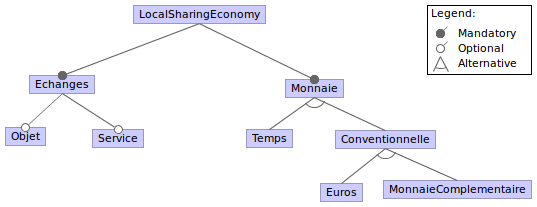
\includegraphics[scale=0.6]{exemple.png}}

Une petite précision est nécessaire pour pouvoir comprendre ce diagramme correctement.  On peut se poser la question des features alternatifs : s'agit-il d'alternatives exclusives ou non ?  Dans ce cas-ci,  nous dirons que oui.  Ainsi,  notre système ne pourra avoir qu'une seule monnaie parmi les choix : Temps,  Euros,  MonnaieComplémentaire.  Conceptuellement parlant,  nous pourrions imaginer un système avec plusieurs monnaies mais cela complexifie assez bien la tâche.

Pour la définition des features,  nous aurions ce qui suit : \\
\textbf{\underline{Local Sharing Economy : }} Economie locale d'échange,  il s'agit d'une communauté dont l'activité principale est l'échange entre personnes d'une zone géographique restreinte. \\
\textbf{\underline{Echanges : }} Action du passage d'un bien ou un service d'une personne à une autre,  en échange d'un montant de monnaie fixé.\\
\textbf{\underline{Monnaie}} Outil de mesure de la valeur d'un bien ou d'un service.
\textbf{\underline{Objet}} Un bien matériel dont on peut définir le propriétaire. \\
\textbf{\underline{Service}} Une action utile pour une personne. \\
\textbf{\underline{Temps}} Unités de temps exprimée en minutes, heures,  jours,  semaines et mois.  \\
\textbf{\underline{Monnaie conventionnelle}} Monnaie représentée sur forme matérielle et n'existant pas naturelement. \\
\textbf{\underline{Euro}} Monnaie officielle de la zone Euro. \\
\textbf{\underline{Monnaie complémentaire}} Monnaie conventionnelle mais non-officielle (non reconnue par les autorités civiles nationales). \\


Ensuite,  nous devons décrire les règles de composition.  Une règle que nous pouvons définir concernerait l'échange de biens et la monnaie utilisée.  En effet,  il semble difficile ou,  en tout cas,  peu logique,  de donner une valeur temporelle à un objet.  Nous pouvons donc décrire la règle que si le feature "Biens" est présent,  alors il faut une feature de type "Monnaie conventionnelle",  équivalent au feature "Biens" est mutuellement exclusif au feature "Temps".  D'une manière plus générale,  les règles de compositions sont souvent de 2 types : featureA \textbf{nécessite} featureB et featureA \textbf{est mutellement exclusif avec} featureB.  Tels que les noms l'indiquent,  la première règle signifie que si on désire intégrer featureA,  alors on doit également avoir featureB intégré.  La seconde règle signifie que l'on ne peut pas avoir featureA et featureB. 

%======== Paragraphe à relire car c'était celui d'en dessous avant.
%====================================================

Pour terminer notre feature model,  nous devons décrire les arguments qui doivent permettre de décider de la présence ou non de chaque feature.  D'abord,  nous voyons que "Echanges" et "Monnaies" sont obligatoires.  Nous n'avons pas le choix car toute économie d'échange local doit avoir défini ces 2 composantes.  Ensuite,  les features "Objet" et "Service" sont optionnels.  Le choix d'inclure un ou les 2 features sera simplement guidé par la réalité du terrain : voulons-nous que les échanges concernent des biens et/ou des services ?  De l'autre côté de notre diagramme,  nous avons la monnaie.  Notre règle compositionnelle nous signale déjà que notre choix sera guidé d'après la présence ou non du feature "Biens".  De plus,  si nous utilisons une monnaie conventionnelle,  le choix d'une monnaie alternative peut être motivé si on désire renforcer l'aspect local de l'économie.  \\

Ceci termine la description d'un exemple de feature model.  Nous avons utilisé un thème lié au mémoire mais,  bien sur,  il s'agit là d'une petite partie de l'analyse qui sera faite plus tard.  Ce chapitre nous a donc permis de mieux comprendre le principe des feature models et nous allons maintenant passer à la suite de la description des outils utilisés pour le mémoire. 

\subsection{Outil : featureIDE}

Pour pouvoir représenter le feature model que nous aurons élaboré,  il va falloir utiliser un outil efficace principalement pour représenter le feature diagram et pouvoir le modifier facilement. 

Au début de l'analyse,  nous avions utilisé une application disponible en ligne et permettant même de sauvegarder les projets sur la base de données du site.  Cet outil se nomme Software Product Line Online Tools \cite{splot}.  Malheureusement,  cet outil est fort simple et ne permet une visualisation que en arborescence textuelle.  Nous nous sommes donc orientés vers un autre outil plus adapté.  Il s'agit d'un module à installer dans l'environnement Eclipse \cite{eclipse} nommé featureIDE \cite{featureIDE}.  Une fois installé,  celui-ci permet de modifier notre feature diagram de plusieurs façon.  La première la plus intuitive est l'environnement graphique.  Ainsi,  les il est très simple d'ajouter / supprimer / modifier un des neouds du diagramme.  On peut aussi modifier directement des contraintes logiques à chaque branchement.  Dans certains cas,  il est intéressant de modifier directement le diagramme en mode "code source".   Ceci est faisable facilement simplement en ouvrant l'onglet "source code".  Le code sourceXML du diagramme apparaît alors et peut être modifié.   
Une fois que le diagramme est terminé,  on peut facilement exporter le résultat au format .PNG.  Les exemples illustrés dans la partie explicative sur les feature models donnent un aperçu du résultat des diagrammes dessinés via featureIDE.  Une autre utilité de ce programme est de pouvoir vérifier que le modèle est cohérent.  Il peut analyser le diagramme afin de voir s'il n'y a pas des éléments contradictoires.

\subsection{Outil : Django}

Lors du développement d'une solution pour BuurtPensioen dans le cadre du cours SINF/INFO 2255,  le groupe 8 (et d'autres) a choisi d'utiliser le framework Django.  Ce choix se comprend assez facilement pour plusieurs raisons.  D'abord,  Django est assez répandu et permet donc d'avoir accès à un grand nombre de ressources d'aide au développement (tutoriels,  FAQs,  forums, \dots ).  Ensuite,  Django permet d'utiliser des extensions très facilement.  Ceci est utile pour rajouter des fonctionnalités sans devoir réinventer la roue.  Nous allons donc aborder maintenant cet outil plus technique et qui sera utilisé pour l'étape de développement de notre framework.  Étant donné l'ampleur de l'outil et l'importance de celui-ci dans le projet,  il est intéressant de passer un peu de temps à se familiariser avec le framework Django.  

\label{django}
Django \cite{django} est un framework écrit en python \cite{python} et destiné à faciliter la mise en place de sites internet.  

D'un point de vue architectural,  un \textbf{projet} django utilise une ou plusieurs \textbf{application(s)}.  Ensuite,  chaque application fonctionne sous le principe Model-View-Controller.  C'est-à-dire qu'on divise l'application en 3 \textit{couches} : le modèle contient les données (classes,  bases de données, ....),  la vue s'occupe de la partie visible par l'utilisateur et enfin la partie controlleur gère la logique de l'application.  Dans le cas d'une application Django,  on décrit les données (=le modèle) dans un seul fichier : models.py.  Celui-ci est utilisé pour générer automatiquement la base de données.  La vue est gérée dans différents fichiers que l'on nomme  \textbf{templates}.  On aura un fichier par page web et Django rajoutera,  aux endroits définis par le code,  les informations issues de la base de données.  En plus des \textbf{templates},  il faut définir les URL qui seront utilisées et préciser quelle fonction va gérer chacune d'elle.  Ceci se fait dans le fichier urls.py.  Enfin,  on décrit le fonctionnement de l'application (couche controlleur) dans un fichier qui porte le nom,  à tort,  views.py.  Ce nom lui a été attribué car il contient,  en fait,  la logique pour chacune des pages de la vue.  Il y a donc un lien fort avec la vue mais c'est bel et bien là que se retrouvera toute la logique du site web.  Dans ce fichier,  on retrouve chacune des fonctions pointées par les URL définies précédemment.  Les fonctions peuvent faire appel ou mettre à jour la base de données,  manipuler les données,  puis les envoyers à un template qui permettra d'afficher le tout à l'utilisateur.  

Afin de voir plus en détails le fonctionnement de Django,  nous allons créer une simple application web.  Étant donné que le sujet de ce mémoire concerne des offres et demandes de biens ou services,  nous allons créer un mini-site qui aura pour but d'enregistrer des offres ou demandes ainsi que de voir la liste des éléments enregistrés.

Après avoir installé Django sur notre machine,  nous pouvons créer notre premier projet.  Une commande crée automatiquement une structure de base.  Nous créons ensuite aussi automatiquement les fichiers et dossiers de notre application.  Il ne reste plus qu'à programmer dans celle-ci.  

D'abord,  concernant la couche "modèle" (données) de notre application,  nous avons simplement des "BusinessUnits" et des "Actors".  Les BusinessUnits représentent les entités vendues ou échangées tandis que les Actors représentent les vendeurs ou acheteurs de notre système.  Chaque BusinessUnit possède les caractéristiques suivantes : un nom,  un vendeur (=Actor),  un acheteur (=Actor) et une date de validation.  Les Actors eux ont simplement un nom.  Nous allons donc décrire ceci dans le fichier models.py : 

\lstset{language=Python,frame=single,keywordstyle=\color{blue},commentstyle=\color{green},breaklines=true}

\begin{lstlisting}
class Actor(models.Model):
	name = models.CharField(max_length=50)

class BusinessUnit(models.Model):
	descr_text = models.CharField(max_length=200)
	vendor_name = models.ForeignKey('Actor',related_name='actor_vendor')
	buyer_name = models.ForeignKey('Actor',related_name='actor_buyer')
	date_validated = models.DateTimeField('validation date')
\end{lstlisting}

Ce code est suffisant et sera utilisé par Django pour générer puis gérer les accès à la base de données.  Une simple commande permet d'appliquer ce schéma à la base de données et directement après,  nous pouvons insérer ou lire les données selon le schéma que nous venons de définir.

Maintenant que le modèle des données est défini,  nous allons passer aux vues (templates) et aux controlleurs (views.py).  Pour essayer d'être le plus clair possible sur le fonctionnement,  nous allons retracer les appels de fonctions au sein du code source.  Ainsi,  étant donné que nous réalisons une application web,  nous allons démarer d'une URL.  Nous allons définir dans l'application Django une URL qui permettra d'accéder à une page reprenant toutes les BusinessUnit présentes dans la base de données.

Pour cela,  nous modifions d'abord le fichier urls.py et définissons comme suit : 

\begin{lstlisting}
from django.conf.urls import url
from . import views

urlpatterns = [
    url(r'^$', views.index, name='index'),
]
\end{lstlisting}

Cette définition permet d'indiquer à Django la fonction utilisée pour gérer l'URL pointant sur l'index de notre application.  La fonction utilisée sera celle donc views.index,  c'est-à-dire la fonction index dans le fichier views.  

Nous devons maintenant définir cette fonction dans le fichier views.py.  Dans cette fonction,  nous devrons récupérer tous les BusinessUnits,  puis choisir un template qui affichera les données,  ensuite créer le contexte,  c'est-à-dire la correspondance entre les données récupérées dans la base de données avec le nom des variables présentes dans le template.  Enfin,  il faut renvoyer à l'utilisateur le mélange des 2 : notre template avec du contenu dans les variables.  Nous verrons juste après le template proprement dit.  D'abord le code de la logique décrite ci-avant : 

\begin{lstlisting}
from django.template import RequestContext, loader
from django.shortcuts import render
from django.http import HttpResponse

from .models import BusinessUnit, Actor

def index(request):

    # On recupere 5 BusinessUnits de la base de donnees
    liste = BusinessUnit.objects.order_by('date_validated')[:5]
   # On cree un contexte avec les donnees recuperees
    context = RequestContext(request, {
        'liste': liste,
    })

   # On charge un template qui sera utilise pour presenter les donnees
    template = loader.get_template('basiceconomy/index.html')

   # On retourne a l'utilisateur le template avec son contexte
    return HttpResponse(template.render(context))

\end{lstlisting}

Il ne nous reste plus qu'à créer notre template dans le dossier "templates" de l'appliaction et à l'endroit que nous avons indiqué,  c'est-à-dire dans le sous dossier basiceconomy/.  Un fichier de template est un mix entre du HTML et du python.  Le HTML représente de la mise en forme finale tandis que le python est utilisé pour insérer des données ou messages divers à partir des variables définies dans le contexte de la page.  A la base,  le code est considéré comme du HTML et lorsqu'on décide d'insérer du python,  on place le code entre \{\% et \%\} ou bien \{\{ et \}\} pour insérer purement le contenu d'une variable.  Le code du template de notre page d'index repenant la liste des BusinessUnits se présente donc comme suit : 

\begin{lstlisting}


    <ul>
    
        <li>{{ bu.descr_text }}</li>
    
    </ul>

    <p>No business units are available.</p>


\end{lstlisting}

Tout ceci étant fait,  il ne reste plus qu'à lier notre application à notre projet afin qu'elle soit accessible.  Pour cela,  il suffit de modifier 2 fichiers dans le dossier du projet : le fichier de configuration (settings.py) dans lequel on indique qu'on utilise notre application,  et le fichier urls.py dans lequel nous indiquons qu'il faut inclure les urls de notre application dans celles du projet en général.  
En guise de résumé de ce petit tutoriel,  nous allons jeter un oeil à l'arborescence finale de notre projet.  A noter que nous avons nommé notre projet "testproject" et notre application se nomme "basiceconomy".  L'arborescence,   au départ du dossier principal du projet,  est la suivante.
\\
\\
\underline{\textbf{.:}} \newline
\textbf{testproject} \newline
\textbf{basiceconomy} \newline
db.sqlite3 \newline
manage.py \newline

A la racine,  nous retrouvons 1 dossier du même nom que notre projet principal ainsi qu'un dossier du même nom que notre application.  Pour chaque application développée pour le projet,  nous créerons un nouveau dossier ici qui portera son nom.  On retrouve aussi le fichier manage.py qui permet d'administrer le serveur django (effectuer les migrations de la base de données,  créer un superuser,  lancer le serveur, \dots )
\\
\\
\underline{\textbf{./testproject:}} \\
\textbf{\_\_pycache\_\_} \\
\_\_init\_\_.py \\
settings.py \\
urls.py \\
wsgi.py \\

Le dossier du même nom que notre projet reprend le code qui le concerne.  Nous n'y avons modifié que 2 fichiers : settings.py dans lequel nous avons renseigné que nous utilisions l'application basiceconomy et urls.py dans lequel nous avons indiqué qu'il fallait inclure les urls de l'application basiceconomy dans les urls du projet général.Le reste des fichiers et dossiers a été généré automatiquement lors de la création du projet.
\\
\\
\underline{\textbf{./basiceconomy:}} \\
\textbf{migrations} \\
\textbf{templates} \\
\textbf{\_\_pycache\_\_} \\
admin.py \\
\_\_init\_\_.py \\
models.py \\
tests.py \\
urls.py \\
views.py \\

Nous sommes maintenant dans le dossier principal de notre application basiceconomy.  Nous avosn commencé par modifier models.py afin d'y décrire notre modèle de données.  Il fallait alors effectuer une migration (au moyen du fichier manage.py présent à la racine du projet) de la base de données.  Ensuite,  nous avons modifié urls.py pour pouvoir lier une url avec une fonction.  La fonction en question est décrite dans views.py et récupèrera un template.  Ce template se retrouve plus loin dans l'arborescence (dans le dossier templates).
\\
\\
\underline{\textbf{./basiceconomy/migrations:}} \\
\textbf{\_\_pycache\_\_} \\
0001\_initial.py \\
0002\_auto\_20150409\_1142.py \\
0003\_auto\_20150409\_1445.py \\
\_\_init\_\_.py \\

Ce dossier est utilisé pour retenir les différentes migrations,  c'est-à-dire les différences entre le modèle décrit dans models.py et la base de données.  Tout ceci est géré automatiquement via une simple commande.
\\
\\
\underline{\textbf{./basiceconomy/templates:}} \\
\textbf{basiceconomy} \\

Les templates sont regroupés dans des sous-dossiers pour des raisons d'organisation.
\\
\\
\underline{\textbf{./basiceconomy/templates/basiceconomy:}} \\
details.html \\
index.html \\

On retrouve finalement nos templates qui,  une fois couplés avec un contexte de données,    permettront d'afficher une page à l'utilisateur.

Ce petit exemple terminé,  nous avons pu avoir un aperçu du fonctionnement global de Django.  

\subsection{Open-source et licences}

Dès le début de l'analyse des besoins,  il est apparu qu'il fallait éviter que l'histoire se répète pour l'outil qui allait être développé. En effet,  d'autres outils existent et certains ont été,  à une époque,  en accès gratuit pour les organisations qui le désiraient.  Mais vu le succès rencontré,  les propriétaires ont repéré l'opportunité de faire du profit et certains outils sont maintenant devenus (parfois partiellement) payants.  La question de la licence d'utilisation a donc été une des premières questions à poser.  

Pour cela,  une rencontre avec le Louvain Technology Transfert Office a été organisée et de bons éléments de réponses ont pu être apportés.   L'idée étant d'analyser ce que l'on désire pour l'avenir de notre application et de choisir une licence appropriée en fonction de ces perspectives pour le futur.

D'abord,  2 catégories de licences existent : les licences propriétaires et les licences open-sources.  Dans les 2 cas,  il faut prêter attention au transfert de licence.  C'est-à-dire du fait qu'utiliser un programme ou un bout de programme dans son propre projet,  peut avoir des conséquences sur la licence de notre projet.  Par exemple,  il se peut que la licence de la bibliothèque utilisée soit transférée à tout notre projet,  si on l'utilise.  De plus,  les questions de la disponibilité du code source ainsi que la possibilité de l'utiliser/modifer gratuitement occupent une place centrale dans la réflexion.  Dans notre cas,  comme dis ci-dessus,  l'inquiétude principale était d'empêcher qu'une personne puisse s'approprier le projet et le rende payant pour les utilisateurs.  Dès lors,  les licences open-source semblent correspondre et parmis elles,  on peut citer la plus connue : GPL (GNU Public Licence).  Cette licence est celle utilisée "par défaut" pour les projets open-source.  Elle semble correspondre car elle ne supporte pas le mélange avec des logiciels propriétaire et oblige à rendre le code de l'application disponible lorsqu'on la distribue.  Elle peut donc empêcher qu'une partie ou  l'entièreté du projet soit privatisée.  Cependant,  nous ne sommes pas au bout de la réflexion.  En effet,  sachant que notre projet prendra très probablement la forme d'un site web,  il est intéressant de voir si une licence n'est pas plus adaptée à cette sitaution.  Pour cela,  le cas de l'AGPLv3 (Affero GNU Public Licence) semble correspondre à nos besoins.  Il s'agit d'une licence basée sur GPL  mais exigeant que,  pour les applications online,  l'accès au code source doit être explicitement référencé quelque part.  Ce système permet d'éviter le cas,  par exemple,  de certains applications Google.  En effet,   l'utilisation de ces systèmes est gratuite mais il n'est techniquement pas possible de récupérer le code source.  Sous licence AGPL,  l'application doit inclure quelque part un lien vers le code source du projet.  

En définitive,  c'est la licence AGPLv3 qui sera choisie pour couvrir le projet de framework.  Ceci permettra aussi peut-être de pouvoir créer une communauté de développement autour du framework afin d'améliorer celui-ci,  à l'instar de Linux et d'autres projets open-source portés par une forte communauté.

Cette section sur les licences clôture ce chapitre à propos des outils utilisés dans le cadre de ce mémoire.  Nous avons également déjà pu,   via les exemples, aborder la thématique des échanges locaux.  Il s'agit du sujet principal du chapitre suivant qui vise à décrire le problème traité dans ce travail.

\section{Problem Statement}

Maintenant que nous sommes bien outillés,  nous allons pouvoir décrire notre problème,  c'est-à-dire notre question de base que nous résoudrons par la suite.  Ce chapitre s'attarde donc à décrire les éléments du problème tels qu'ils ont été présentés au début ou pendant la réalisation de ce mémoire.  Tout d'abord,  nous allons décrire le cas de l'organisation BuurtPensioen et ses besoins,  qui furent le point de départ du mémoire.  Ensuite,  nous décrirons le logiciel créé par un groupe d'étudiants du cours LSINF/INFO2255 qui a été présentée en décembre et qui a servi de base pour être transformé et devenir le framework final.

\subsection{BuurtPensioen}

BuurtPensioen \cite{buurtpensioen} (\"pens('i)ons voisin\",  en français) est un projet néerlandophone basée à Bruxelles issue de la collaboration entre diverses associations de la capitale.  Ce projet regroupe une communauté de membres qui s'entraident mutuellement.  Le principe est le suivant.  Dans la vie,  nous sommes assez autonomes pendant l'âge adulte mais cela diminue avec l'âge.  Ainsi,  les personnes plus âgées deviennent dépendant de l'aide d'autres personnes.  C'est dans ce sens que le système de pensions a été créé : on épargne de l'argent lorsqu'on est en âge de travailler et on le reçoit en retour une fois que l'on prend sa retraite.  L'organisation BuurtPensioen est basée sur ce principe mais ne fonctionne pas avec de l'argent mais plutôt avec du temps.  En effet,  lorsque quelqu'un rend un service à une autre personne,  on compte en minutes ou en heures,  le temps que ce service a pris.  La personne qui a aidé "reçoit" alors ce temps et peut le cumuler.  Avec en perspective d'avoir une certaine réserve de temps pour le moment ou cette personne ne sera plus en capacité de se débrouiller seule.  Elle pourra alors utiliser son "capital-temps" afin de se faire aider.

Ce système a été mis en place suite à un constat que les aides organisées par l'état pour les personnes âges sont de moins en moins présentes en Belgique et,  au delà de ce constat financier,  beaucoup de ces mêmes personnes sont également isolées du reste du monde.  La solution proposée par BuurtPensioen permet d'aider la personne âgée mais cette aide est aussi une occaison de reconnecter la personne avec le reste de la société.   

Un projet pilote a été lancé en novembre 2013 dans la commune de Neder-over-Heembeek.  Celui-ci a remporté un vif succès et il est envisagé de créer d'autres projets dans ou aux alentours de Bruxelles.  

Cependant,  le projet BuurtPensioen aimerait d'abord se munir d'un outil plus automatisé avant d'élargir son terrain d'action.  Pour cela,  une collaboration avec l'UCL a été mise en place en 2014.  Le professeur Kim Mens,  enseignant du cours "SINFINFO 2255 Projet de développement logiciel",  a participé à l'élaboration d'un cahier de charges pour la création de cette plateforme ( voir Annexe 1 \ref{bpse} ).  L'objectif étant de proposer ce sujet comme projet pour le cours pré-cité.  
\newline
\newline
Pour se faire une petite idée du style d'outil qui a été demandé par le consortium Buurtpensioen,  nous allons parcourir rapidement quelques éléments clés de ce cahier des charges.

\begin{description}

\item [Membres]
Le logiciel créé doit gérer un système de membres de différent types.  D'abord,  les membres "normaux".  Il s'agit des utilisateurs finaux de l'application,  c'est-à-dire les personnes âgées ainsi que celles qui les aident.  Ensuite,  des membres du type "administratif",  c'est-à-dire des gestionnaires du projet BuurtPensioen.  Ces gestionnaires peuvent être de 2 niveaux : soit administrateurs d'une région géographique (branches),  soit administrateurs du système dans son entièreté.

\item [Crédits]
Chaque membre doit posséder son propre "compte" de temps accumulé.  Celui-ci représente la pension du membre,  c'est-à-dire la somme des services qu'il a déjà rendu,  valorisés en unité de temps,  et qui pourra être utilisé en cas de besoin dans l'avenir.  De plus,  un système de dons doit être mis en place afin de permettre à des membres d'offrir une partie ou l'entièreté de son crédit à une autre personne.

\item [Branches]
La solution proposée doit inclure un système de "branches".  Cette appellation désigne des antennes locales de l'organisation,  que les membres pourraient rejoindre.  Les antennes locales (= branches) représentent des zones géographiques.  
Chaque branche possède,  dans le système,  des informations qui lui sont propres telles que son adresse,  le nom de l'administrateur de cette branche,  etc.

\item [Offres-Demandes]
Le système aura bien sur pour but de mettre les membres en relation sur base des offres et demandes qu'ils encoderont.  Ainsi,  les personnes dans le besoin seront invitées à encoder leurs demandes dans le système en fournissant les informations nécéssaires pour le service demandé,  c'est-à-dire le moment où le sevice est demandé,  le type de service,  le temps que cela prendrait, etc.

\item [Divers]
Diverses exigences sont également à prendre en compte et concernent l'application dans son entièreté.  Premièrement,  étant donné que le système sera utilisé par des personnes pouvant ne pas être habituées à l'informatique,  il faut que l'application soit facile d'utilisation notamment via une interface simple.  Ensuite,  la solution proposée doit prendre en compte les aspects de sécurité afin que les données encodées par les membres ne soient pas dérobées ou altérées.  Enfin,  il est demandé de mettre en place un système de statistiques à propos des membres ainsi que de l'utilisation (nombre d'offres/demandes,  temps de réponse à une demande, \dots ) et d'autres fonctionnalités de plus petite utilité tels qu'une possibilité de lien avec Facebook,  l'utilisation de Google Maps, \dots .

\item [Statistiques pour la VUB]
Lors d'une rencontre avec Liesbeth De Donder,  doctorante à la VUB,  nous avons également abordé le thème des statistiques qui devraient être accessibles dans l'application.  En effet,  l'université de Bruxelles aimerait avoir la possibilité de récolter et traiter des données concernant l'utilisation et les utilisateurs des systèmes tels que celui qui doit être développé pour Buurtpensioen.  Au départ,  les statistiques ne sont que l'une des fonctionnalités demandées pour Het Buurtpensioen.  Mais sachant que des acteurs extérieurs sont intéressés par les statistiques,  nous pouvons considérer que les statistiques sont un point important de l'application.  Du moins,  pour le framework développé puisque cet "appui" concernant les statistiques ne fait pas partie du cahier des charges initialement donné comme référence de base aux étudiants du cours de Software Development Project.   

\end{description}

Pendant tout le premier quadrimestre,  les étudiants du cours ont donc travaillé à l'élaboration d'une solution répondant à ce cahier des charges.  Le travail étant réalisé par groupes de 6 à 8 étudiants,  il a résulté de ce cours plusieurs propositions de solutions.  Parmi celles-ci,  la solution du Groupe 8 a été celle qui a le plus retenu l'attention de Katleen Deruyter,  personne de contact de BuurtPensioen pour tout le processus de collaboration entre l'UCL et l'organisation.  Cette solution a été analysée et utilisée pour la deuxième partie du mémoire (réalisation du framework).  C'est pourquoi nous allons maintenant décrire rapidement la solution proposée.


\subsection{Solution proposée dans le cadre du cours LSINF/INFO 2255}

La solution proposée par le Groupe 8 du cours LSINFINFO2255 de 2014-2015 consiste en un site web utilisant Django (voir section \ref{django}).  Nous allons parcourir rapidement l'application développée afin de mieux se rendre compte du genre d'outil désiré.

Commençons par la page d'accueil du site internet.  

\vspace{1cm}
\fbox{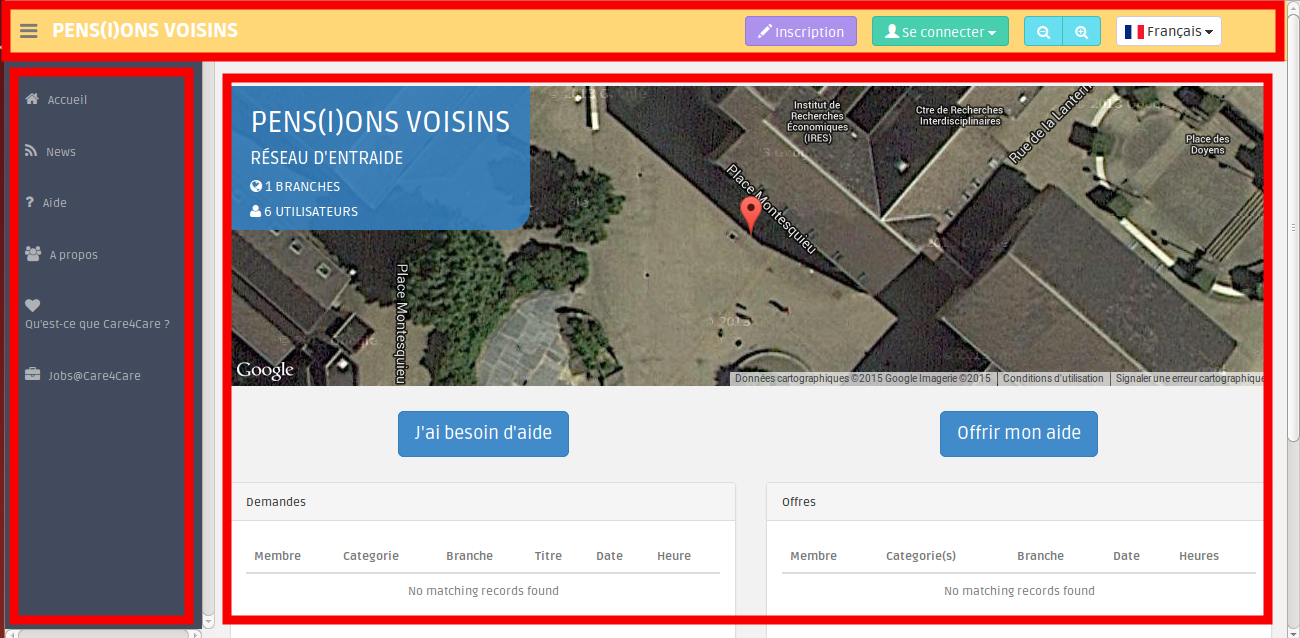
\includegraphics[scale=0.30]{gr8home1.png}}
\vspace{1cm}

On observe (en rouge) 3 zones principales sur l'écran : le menu de navigation sur la gauche,  le menu de connexion dans la barre supérieure et la zone de contenu sur le reste de la page.  
Tout d'abord,  le menu de connexion dans le haut de la page permet à l'utilisateur de s'enregistrer ou de s'identifier s'il est déjà inscrit.  On peut également changer la langue du site internet.  Notons que toutes les langues ne sont pas encore implémentées à 100\%.  
Ensuite,  le menu à gauche peut varier selon qu'on est connecté ou non.  Il permet de naviguer entre les différentes pages principales du site.  
Enfin,  la partie contenu du site affiche,  à l'accueil,  une carte Google Maps reprenant les branches existantes localisées par une pipette rouge,  et juste en dessous,  deux tableaux reprenant chacun la liste des offres et la liste des demandes qui ne sont pas encore complétées.  

Si on suit un scénario classique sur le site,  on peut commencer par se rendre sur la page d'inscription au site afin de voir à quoi celle-ci ressemble.

\vspace{1cm}
\fbox{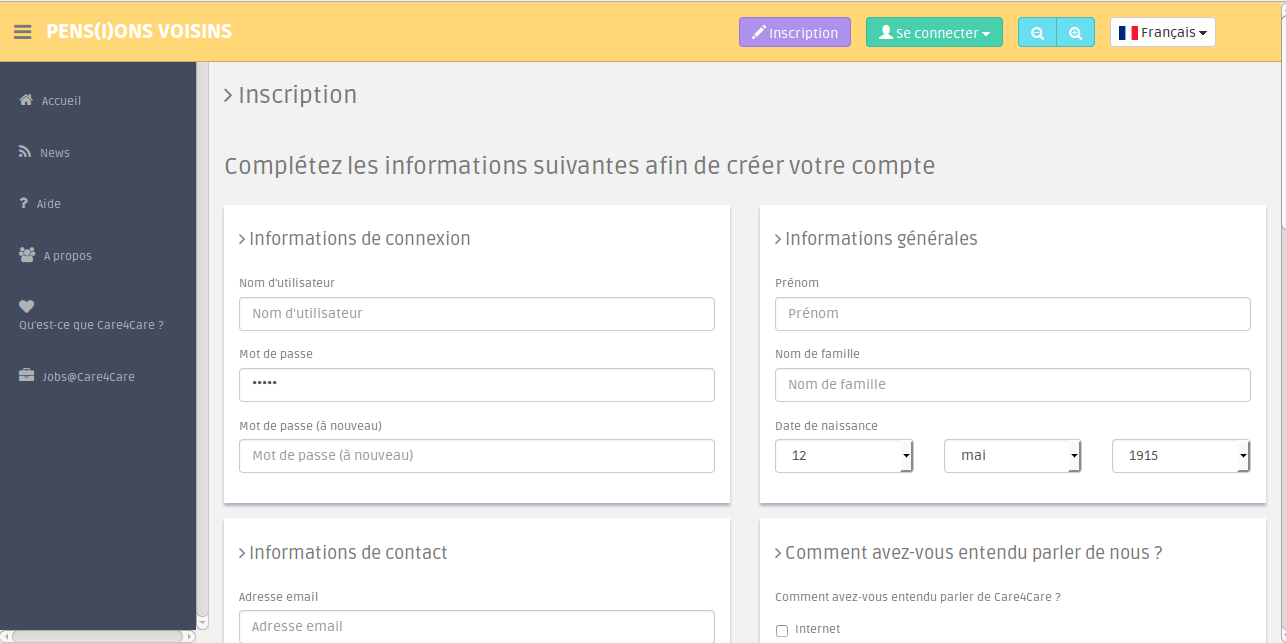
\includegraphics[scale=0.30]{gr8inscr.png}}
\vspace{1cm}

Sur cette page,  on accède au formulaire d'inscription demandant de renseigner des données d'identification habituelles telles que nom d'utilisateur et mot de passe,  adresse email et autres mais il est également demandé de choisir une branche (= une antenne locale du projet) que l'on rejoindra dès le début.  

Après s'être enregistré puis connecté,  nous pouvons retrouver nos informations sur la page Profil.

\vspace{1cm}
\fbox{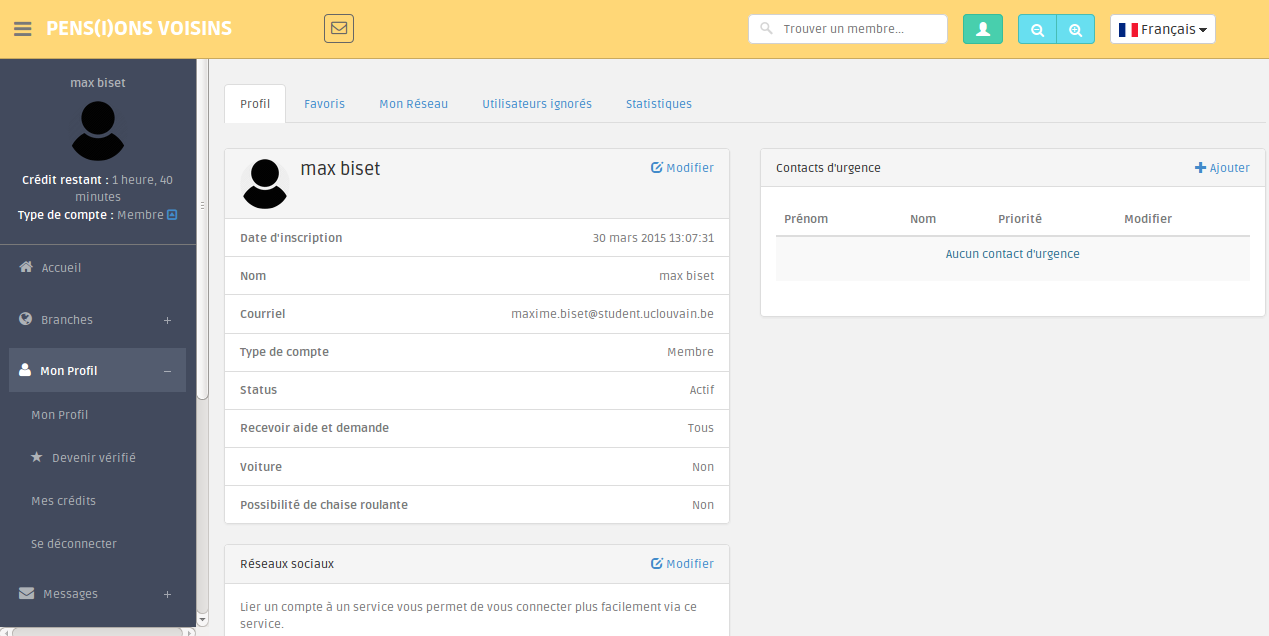
\includegraphics[scale=0.30]{gr8profil.png}}
\vspace{1cm}

Ici,  on retrouve les informations encodées lors de l'inscription mais aussi un accès à d'autres données modifiables telles que les listes d'utilisateurs favoris ou ignorés ainsi que l'accès au statistiques du compte.

Il nous reste maintenant à attaquer le fond même du site,  c'est à dire les échanges.  Pour cela,  nous pouvons analyser de plus près la page d'accueil.  

\vspace{1cm}
\fbox{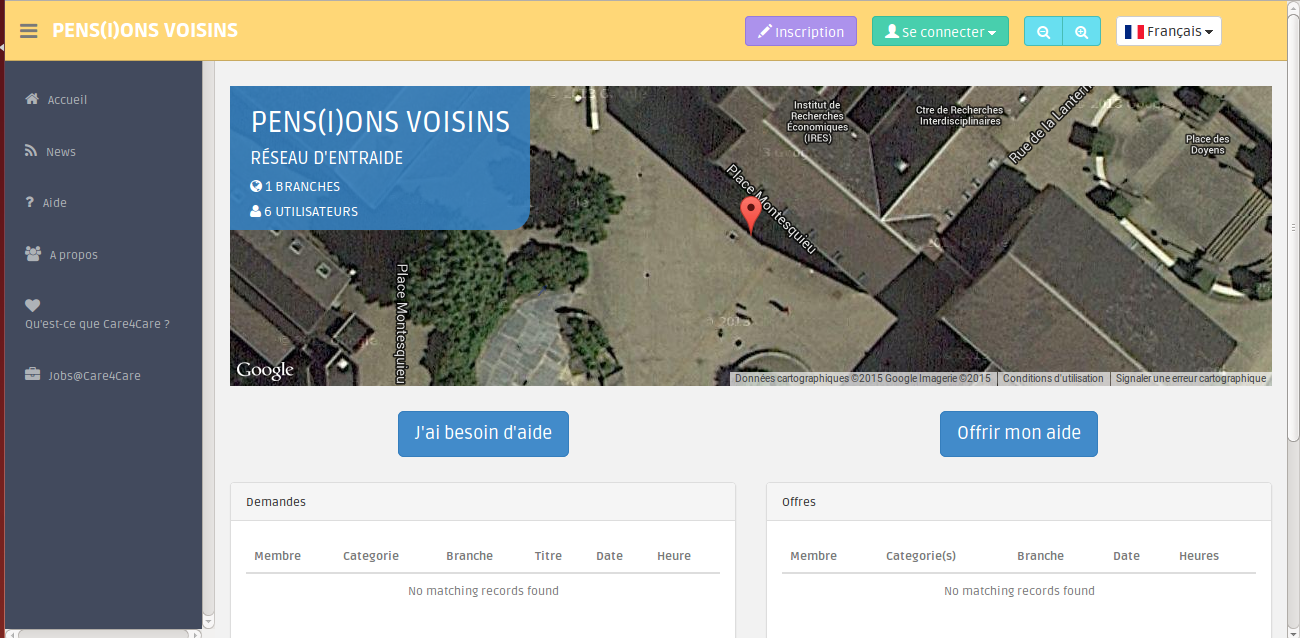
\includegraphics[scale=0.30]{gr8home.png}}
\vspace{1cm}

On remarque sur cette page que 2 catégories existent sur le site : les offres d'aide et les demandes d'aide.  Celles-ci apparaissent dans deux parties de l'écran.  Un simple bouton permet également d'enregistrer une demande ou une offre.  

Nous allons maintenant voir un aperçu d'une page destinée à encoder une demande d'aide.

\vspace{1cm}
\fbox{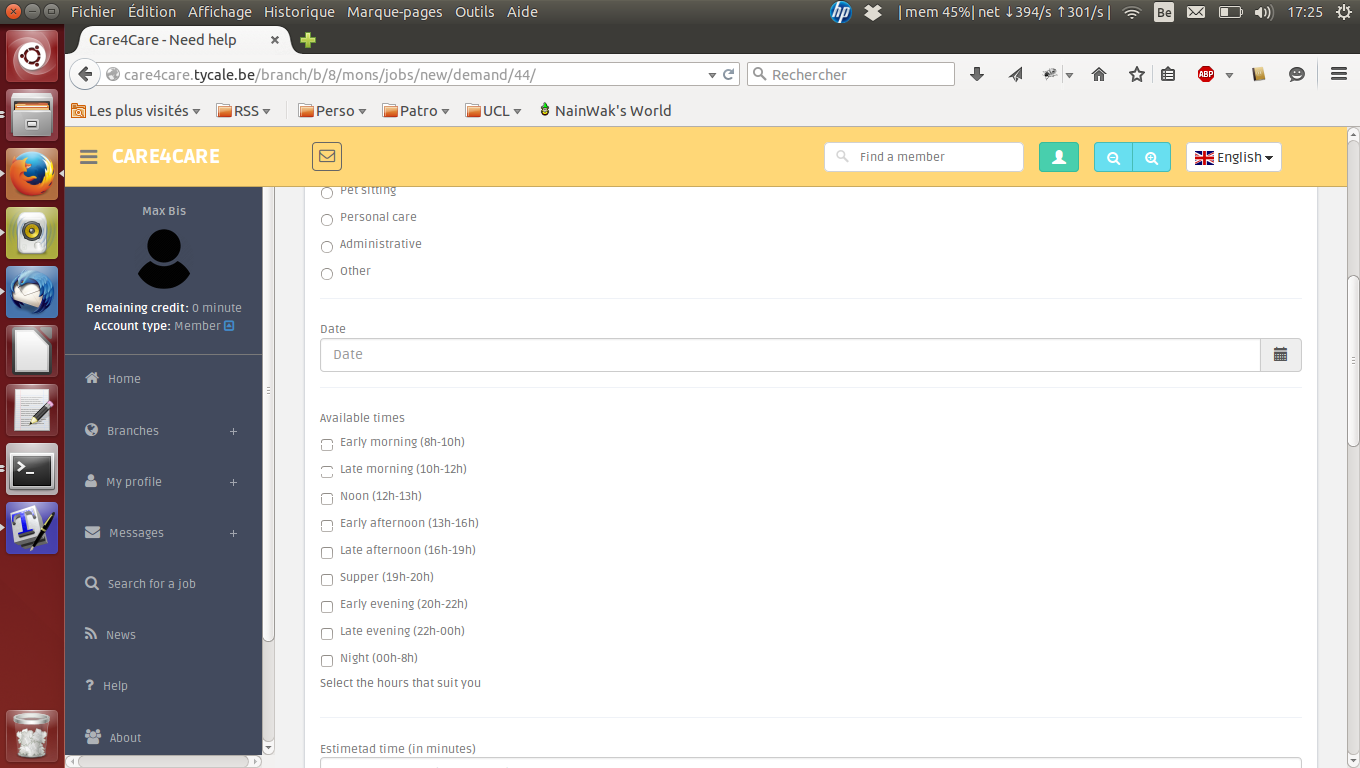
\includegraphics[scale=0.30]{encoder.png}}
\vspace{1cm}

Sur cette page,  l'utilisateur est invité à encoder les informations liées aux service recherché.  Pour cela,  il peut choisir un type de service,  le moment où celui-ci doit avoir lieu ainsi que le lieu.  Il est également possible d'entrer un titre et une description du service.  Après que la demande de service soit encodée dans le système,  elle apparait dans la liste des demandes non remplies.  Lorsqu'un utilisateur répond à la demande,  l'initiateur de celle-ci est averti et peut valider la réponse.  Une fois le service rendu,  la demande n'est plus affichée dans la liste.

Nous avons ainsi pu faire un rapide tour de l'application créée par les étudiants du cours de Software Development Project.

\subsection{Autres organisations existantes}
\phantomsection
\label{autresOrgas}
Après avoir observé ce cas principal de BuurtPensioen,  nous allons aborder rapidement quelques autres organisation et outils existants.  Ceci permet de se rendre compte du paysage des applications possibles pour un framework tel que nous voulons le développer.  Dans le domaine des échanges locaux,  ces informations ont été récoltées selon 2 cannaux : d'une part,  une réunion avec divers représentants d'organisations semblables à BuurtPensioen qui a eu lieu en octobre 2014 et d'autre part,  diverses recherches sur internet.

\begin{description}

\item [Cyclos (http://www.cyclos.org/)]

Cyclos est un logiciel d'online et mobile banking.  Il ne s'agit,  ici,  que d'un outil qui peut être utilisé par des organisations.  Cet outil est adaptable à plusieurs situations et permet d'utiliser diverses monnaies dont des monnaies complémentaires.  Il est développé par le réseau Social TRade Organisation (\cite{STRO}) et plusieurs versions existent : une gratuite et open-source téléchargeable sur le site web de Cyclos,  un système de services Cyclos pour les communautés locales (il est possible de créer son initiative locale via le site officiel de Cyclos),  et enfin une version "pro" destinée aux grandes organisations avec des prix variant de 1000 à 3000 euros de frais d'abonnement par an,  voire plus selon négociation lorsque les organisations sont de très grande taille.  
Enfin,  l'outil Cyclos est sous licence GNU General Public Licence.

\item [System d'Entraide Local (SEL) (www.sel-lets.be/ )]

Le SEL est en même temps un outil et des organisations.  Ce site propose aux communautés de s'inscrire chez eux et de leur fournir les services d'un outil permettant l'échange de services.  Ces derniers sont catégorisés dans diverses thématiques.  Chaque communauté possède son minisite sur lequel les utilisateurs peuvent s'enregistrer pour encoder leurs offres et demandes de services.  Les services vont du ménage au bricolage en passant par l'éducation et l'apprentissage.  

\item [QOIN (http://www.qoin.org)]
\phantomsection
\label{QOIN}

QOIN est une entreprise de services de management et d'informatique destiné à la mise en place de communautés locales de monnaies alternatives.  Dans ce cadre,  cette organisation a développé 2 logiciels qui sont utilisés dans la région d'Amsterdam.  Le premier logiciel,  TradeQoin,  est destiné aux petites et moyennes entreprises qui se rendent des services entre elles.  Le second,  ShareQoin,  est utilisé par 10 monnaies alternatives différentes et est destiné à des personnes physiques.  

\item [Troeven.be (https://www.troeven.be/)]
Troeven est un projet en phase de test mené dans la commune de Turnhout (province d'Anvers) et qui utilise l'outil TradeQoin (défini juste avant).  Ce projet utilise comme monnaie des "troeven" ("atouts" en français) et n'est disponible qu'en néérlandais.

\end{description}

Nous avons listé ici quelques outils et organisations qui ont servi de sources d'informations pour ce mémoire.  L'objectif a été d'avoir un aperçu de ce qui existe au niveau des outils pour gérer des projets du même genre que Buurtpensioen ainsi que d'autres projets existants.  

Étant donné que nous allons développer un framework,  la question se pose de savoir quel sera le logiciel d'origine qui va être utilisé comme base pour le développement de ce framework opensource qui pourrait être appliqué,  par exemple,  au cas du projet Buurtpensioen.  Notons que,  dans la pratique,  cette question s'est posée après l'analyse du domaine pour des raisons de timing mais il semble opportun de répondre à cette question ici,  après avoir détaillé les systèmes existants.  
Pour répondre à la demande d'un framework,  2 propositions ont été envisagées pour servir de base : l'outil Cyclos ou celui développé par le groupe d'étudiants et destiné à Buurtpensioen.   En effet,  ces 2 logiciels sont open source et peuvent donc être ré-utilisés.  L'avantage de Cyclos est qu'il possède de nombreuses fonctionnalités (mais pas toutes aceessibles dans la version téléchargeable).  Le second outil,  quant à lui,  a été choisi parmi plusieurs solutions comme étant celle qui répondait le mieux aux demandes de Burrtpensioen,  une des utilisations finales possibles du framework.  C'est d'ailleurs cet argument là qui va faire pencher notre choix car Cyclos est un logiciel à paramétrer tandis que la solution des étudiants est un logiciel fonctionnel prêt à l'emploi.  Cela permet d'économiser une étape supplémentaire pour le développement du framework.  Le choix est donc fait de partir de la solution développée par le groupe d'étudiants pour développer un framework plus global.

Ceci clôture le chapitre sur l'explication du problème à résoudre.  La prochaine étape consiste à analyser de plus près le domaine dans lequel nous allons devoir développer notre framework.  




\section{Approche}

Pour faire face au problème décrit dans le point précédent,  une méthode en plusieurs étapes est nécessaire.  
Tout d'abord,  comme dans la plupart des projets informatiques,  il est important de réaliser une analyse du domaine.  Cependant,  une analyse du domaine "classique" ne conviendrait pas pour le problème tel que décrit ci-dessus.  En effet,  l'objectif étant de réaliser un logiciel applicable à plusieurs organisations ayant chacune ses particularités,  l'analyse doit être faite dans le but de développer,  par la suite,  un framework.  Pour cela,  on fera d'abord un survol du domaine en définissant les principaux concepts puis  nous réunirons un maximum d'informations dans un feature diagram.  Celui-ci permettra de mettre en avant les différentes composantes et possibilités du système et de son outil.  De plus,  ce diagramme est accompagné de contraintes entre les différentes composantes.  Ceci permet d'éviter de définir une application dont certaines parties ne sont pas compatibles entre elles.  Enfin,  lors du développement,  le feature diagram est une bonne source d'organisation.  En effet,  certains features pourront correspondre à des parties "indépendantes".  Cette étape peut donc amener déjà des repères à l'instar de l'étape du design dans une analyse plus traditionnelle.
Ces étapes d'analyse amènent une bonne compréhension du domaine dans lequel nous travaillons ainsi qu'un premier pas vers la construction d'un framework qui devrait répondre aux besoins des différents cas existants.  

La seconde étape pour résoudre le problème posé va consister à partir de l'analyse réalisée et du logiciel choisi comme base de départ,  pour développer le framework qui devra répondre aux exigences définies.  Dans la pratique,  un framework est rarement développé "from scratch",  c'est-à-dire à partir de rien.  Généralement,  un ou plusieurs outils existent déjà et ceux-ci sont analysés et refactorés afin de produire une version plus générique de l'applicaiton.  Nous avons déjà abordé le choix de l'application de base lors de l'explication du problème.  Une fois cette base choisie,  il faut se réapproprier le résultat du travail du groupe d'étudiants et analyser l'architecture ainsi que les fonctionnalités et leur implémentation.  Ensuite,  il faut se nourrir d'autres cas qui n'étaient pas prévu à la base dans le logiciel développé afin de les intégrer au framework.

La dernière étape pour répondre au problème posé consiste à valider la solution proposée.  Pour cela,  nous allons prendre 2 cas suffisamment opposés et essayer de les implémenter au moyen du framework produit.  Le premier cas sera BuurtPensioen avec les fonctionnalités développées par le groupe choisi au début du développement.  Le second cas sera tentera d'instancier le framework de la façon la plus opposée possible au cas de Buurtpensioen.  Par exemple,  comme BuurtPensioen fonctionne avec une monnaie temps,  on peut vérifier ce feature en ne prenant aucune monnaie car ne pas utiliser de monnaie entraîne plus de changements que changer de types (pas de crédits dans le compte utilisateurs,  pas de calcul à la fin de l'échange,  etc).


\section{Analyse du domaine}

Notre problème étant posé,  nous pouvons maintenant attaquer l'analyse du domaine.  Celle-ci se fera en plusieurs étapes où chacune d'elles appliquera le fameux dicton \textit{diviser pour mieux régner}.  En effet,  dans chaque partie de l'analyse,  nous allons scinder le problème de base en unités plus petites et donc plus faciles à maitriser et définir.  D'abord,  nous allons définir  le vocabulaire de notre domaine afin de bien préciser la signification des termes utilisés.  Après cela,  nous allons analyser le feature model développé pour décrire notre domaine afin d'avoir une vue assez complète de notre sujet,  tout en gardant en tête que l'objectif sera de développer un framework basé sur ce modèle.  

\subsection{Dictionnaire des termes - Glossaire}
\label{dicoTermes}
Tous les termes repris ci-dessous sont définis dans le cadre de notre étude de cas.  Certains termes peuvent être interprétés autrement dans d'autres contextes.

\begin{description}

\item [Économie Locale de Partage (Local Sharing Economy)]
Ce terme désigne tout système organisé d'échange de biens et/ou de services à une échelle locale entre différents utilisateurs,  le tout régit par une organisation qui centralise les échanges.

\item [Organisation]
Nous appelerons organisation l'institution ou plus simplement l'ensemble des personnes dont l'une des missions est de gérer une ou plusieurs économies d'échange local.  

\item [Utilisateur]
Un utilisateur est une personne physique ou morale qui participe aux échanges d'une économie locale de partage.  Lorsqu'un utilisateur participe à un échange,  il peut être fournisseur ou bénéficiaire.  

\item [Fournisseur]

Le fournisseur d'une transaction est l'utilisateur qui prestera le service ou bien possède l'objet avant que la transaction ait lieu.  A la fin de la transaction,  celui-ci reçoit un montant (qui peut être nul) déterminé de monnaie mais ne possède plus l'objet échangé.

\item [Bénéficiaire]

Le bénéficiaire d'une transaction est l'utilisateur qui demande la réalisation du service ou bien ne possède pas l'objet avant que la transaction ait lieu.  A la fin de la transaction,  celui-ci donne un montant (qui peut être nul) déterminé de monnaie mais possède l'objet échangé.

\item [Échange - Transaction]

Une transaction implique 2 utilisateurs différents.  L'un endosse le rôle de fournisseur et l'autre celui de bénéficiaire.  Les 2 utilisateurs se mettent volontairement d'accord sur les conditions régissant l'échange.  D'une part,  le fournisseur accepte de fournir un bien ou service au bénéficiaire.  D'autre part,  le bénéficiaire accepte de céder une quantité fixée de monnaie au fournisseur.  

\item [Monnaie]
\label{dicoMonnaie}

Dans le cadre des Local Sharing Economy,  une monnaie est un outil destiné à faciliter les échanges.  Une monnaie porte un nom et doit être quantifiable.  Une quantité de monnaie représente la valeur d'un bien ou d'un service que le bénéficiaire doit débourser pour l'échange et que le fournisseur recevra à la fin de l'échange.  A titre de comparaison,  nous pouvons analyser l'apport de la monnaie par rapport au système de troc.  Dans un échange de type troc,  le fournisseur offre un bien ou service au bénéficiaire et ce dernier offre également un bien ou service au fournisseur.  Les 2 utilisateurs jouent donc les 2 rôles en une seule transaction.  Avec une monnaie,  on permet de ne jouer qu'un seul rôle par transaction.  Ceci est possible grâce au fait qu'on échange d'abord de la monnaie et qu'on peut l'utiliser plus tard pour une autre transaction.   

\end{description}

\subsection{Feature model}

Nous arrivons maintenant au coeur de l'analyse avec la description de notre feature model.  Pour le réaliser,  nous nous sommes inspirés d'un modèle de développement de logiciels,  plus précisément du modèle de développement en spirale.  Les étapes : l'analyse de l'existant,  l'analyse de ses features,  la mise à jour du modèle et enfin la validation du modèle.  Ainsi,  le modèle a d'abord été élaboré en reprenant peu de cas de figure.  Plus particulièrement,  juste avec le cas de BuurtPensioen.  Ensuite,  après documentation des autres systèmes et organsiations existants,  le modèle a été revu et augmenté.  
Pour décrire notre modèle,  nous allons d'abord analyser l'aspect global du feature diagram,  c'est-à-dire la représentation graphique de notre modèle.  Ensuite,  nous parcourerons l'entièreté de celui-ci et définirons plus précisément chaque feature ainsi que ses caractéristiques et sa justification.  Enfin,  nous décrirons les règles de composition du modèle.  

\subsubsection{Feature diagram}

Avant de rentrer dans l'analyse proprement dite,  nous allons vite rappeler les conventions utilisées dans le diagramme pour représenter des liens logiques entre les features.  Une petite légende est visible sur le coté droit du schéma mais celle-ci n'est pas assez explicite.  Ainsi,  à chaque fois que nous arrivons à un noeud de l'arbre,  nous pouvons raisonner comme suit.  Si le feature sur lequel on se trouve est inclut dans le système,  alors si le lien de notre feature vers ses fils : 
\begin{enumerate}
\item{est composé d'un arc de cercle vide,  alors 1 et 1 seul fils est possible ;}
\item{est composé d'un arc de cercle rempli,  alors 1 ou plusieurs fils sont possibles ;}
\item{n'a pas de décoration,  alors certains fils seront obligatoires (ceux surmontés d'un cercle plein) et d'autres seront optionnels (ceux surmontés d'un cercle vide).}
\end{enumerate}

Prenons un simple exemple pour illustrer ce fonctionnement : \\

\begin{minipage}{0.25\linewidth}
$\vcenter{\hbox{\fbox{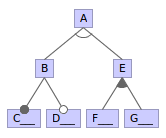
\includegraphics[scale=0.6]{exempleCardinalites.png} } }}$
\end{minipage}
\begin{minipage}{0.7\linewidth} 
Dans ce schéma,  inclure le feature A impose de devoir choisir entre le feature B ou E.  Si on prend B,  alors on sera obligé d'inclure C et on pourra (mais pas obligatoirement) include D.  Si on choisit E,  alors on est obligé d'inclure au moins 1 feature parmi F et G,  sans distinction en favoriser un en particulier.
Ceci étant clarifié,  nous allons analyser,  en plusieurs étapes,  le feature model général d'une Local Sharing Economy.  Etant donné la largeur du diagramme,  celui-ci est découpé en 2 parties.  
Le dessin de gauche correspond à la partie gauche du diagramme.
\end{minipage}

$\vcenter{\hbox{\fbox{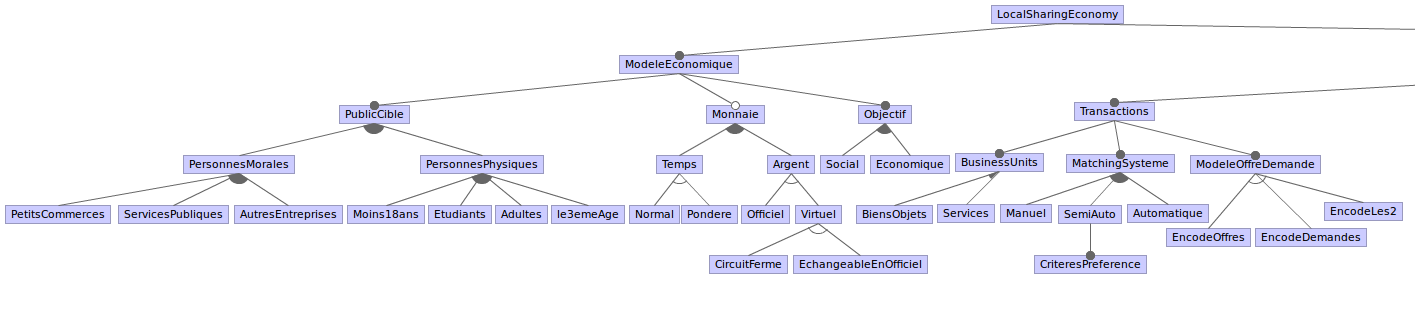
\includegraphics[scale=0.38,angle=90]{fmGenP1.png} } }}$ \hspace{3 cm}
$\vcenter{\hbox{\fbox{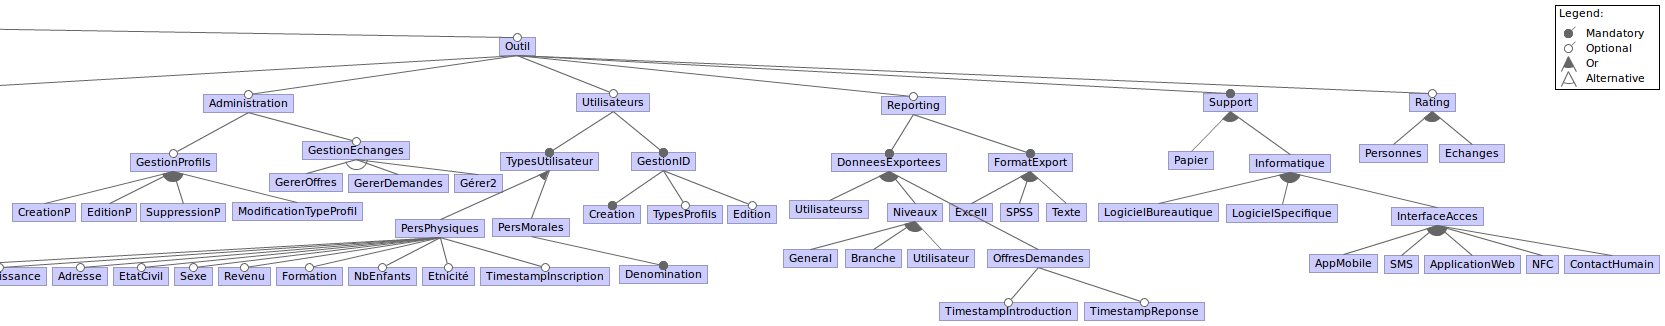
\includegraphics[scale=0.38,angle=90]{fmGenP2.png} } }}$

Une première observation à faire est la découpe en deux parties de notre diagramme.  On retrouve,  dans la partie gauche,  la description du modèle économique et dans la partie droite,  la description de l'outil utilisé.  Les features du modèle économique sont utiles car l'analyse des logiques sous-jacentes à une organisation permet de restreindre les features qui pourront ou non être présents dans l'outil.  De plus,  notre feature model est utilisé comme outil principal pour l'analyse du domaine.  La description du modèle économique permet donc de se rendre compte des possibilités de réalités de différentes organisations.  

Le modèle économique permet d'éclaircir 3 thèmes principaux qui sont le public cible du système,  la monnaie utilisée et l'objectif global du système.  L'outil,  quant à lui,  permet de décrire plusieurs types de fonctionnalités qui peuvent,  ou pas,  être présentes dans un outil de gestion d'une Local Sharing Economy.  Entre autres,  la façon dont les échanges sont gérés,  l'administration possible au sein du système,  les comptes utilisateurs,  les statistiques,  ect.  

\subsubsection{Définition et justification des features}

Nous allons parcourir notre arbre des features selon la méthodologie Depth First Search.  Notons que certains features"de détail"  ne sont pas repris ici.  Une description plus complète peut être trouvée dans les annexes \ref{featureDescr}.

\begin{description}

\item [LocalSharingEconomy]
\underline{Déf. :}  Une économie d'échange local est un système organisé dont l'objectif principal est de promouvoir des échanges de biens et/ou de services dans une zone géographique limitée.  Par exemple,  BuurtPensioen favorise les échanges locaux via l'adhésion à une branche.  Par contre,  lystème des SEL est un système centralisé auquel des communes peuvent s'inscrire.   Notons également que plusieurs expresssions désignent ce genre d'organisation/projet : organisation d'échange social,  économie locale d'échange,  économie d'échange local,  etc.  Ces termes désignent tous les systèmes que nous décrivons.
\\ \underline{Justif. :}  Ce feature est la racine de l'arbre,  ne pas l'inclure signifierait que l'organisation analysée ne peut pas correspondre à l'analyse proposée ici.
\newline

\item [ModèleEconomique]
\underline{Déf. :}  Le modèle économique d'une économie d'échange local correspond aux caractéristiques de l'organisation telle qu'elle est vécue,  indépendamment de l'outil utilisé.
\\ \underline{Justif. :}  Ce feature est obligatoire car toute analyse d'une économie d'échange local doit être d'abord décrite avant de pouvoir s'intéresser à l'outil.
\newline

Nous arrivons maintenant dans le premier sous-arbre : \textbf{PublicCible}.
\newline
\begin{center}
\fbox{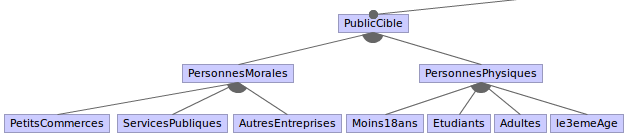
\includegraphics[scale=0.5]{PublicCible.png}}
\end{center}

\item [PublicCible]
\underline{Déf. :}  Le public cible d'une économie d'échange local correspond aux acteurs autorisés à participer aux échanges dans l'organisation.
\\ \underline{Justif. :}  Ce feature est obligatoire car l'organisation n'a pas de sens s'il n'y a pas d'acteurs définis.  Ainsi,  il est obligatoire de sélectionner au moins 1 des fils mais il peut en avoir de plusieurs types.  
\newline

\item [PersonnesMorales]
\underline{Déf. :}  Une personne morale est une construction juridique.  On place dans cette catégorie d'acteurs toutes les entités,  institutions,  organisations et autres groupes considérés comme des acteurs du système.  
\\ \underline{Justif. :}  Certaines organisations permettent,  par exemple,  à des entreprises de faire des échanges entre elles.  Il peut aussi s'agir d'acteurs du service public.  La distinction entre personne morale et physique est nécessaire car cela pourra avoir des répercutions sur l'outil utilisé d'une part pour les fonctionnalités accessibles et d'autre part pour la représentation des données.  Ainsi,  une personne physique pourrait être identifiée par ses nom,  prénom et date de naissance tandis qu'une personne morale ne requièrerait qu'une dénomination générale. 
\newline

Parmi les personnes morales,  on distingue les \textbf{petits commerces},  les \textbf{services publics} et les \textbf{autres entreprises}.

%\item [PetitsCommerces]
%\underline{Déf. :}  Ce feature regroupe les personnes morales de type privé et de petite taille (PME,  indépendants,  \dots )
%\\ \underline{Justif. :}  Etant donné la visée géographique des systèmes d'échange local,  il est tout à fait envisageable qu'une organisation permette,  par exemple,  aux artisans locaux de participer aux échanges.  
%\newline
%
%\item [ServicesPublics]
%\underline{Déf. :}  Les services publics sont toutes les institutions reconnues juridiquement comme agissant pour l'intérêt général.
%\\ \underline{Justif. :}  Des institutions publiques locales peuvent être impliqués dans l'oganisation.  Par exemple,  une commune pourrait faire un appel aux volontaires pour participer à une campagne de nettoyage de la commune.  
%\newline
%
%\item [AutresEntreprises]
%\underline{Déf. :}  Certains acteurs d'un système d'échange peuvent ne pas être des petits commerces ni services publics.  Par exemple,  une multinationale qui désire insérer sa filiale locale dans l'organisation.
%\\ \underline{Justif. :}  Ce feature permet de prendre en compte les acteurs qui ne seraient pas repris dans les cas pré-cités.  
%\newline

\item [PersonnesPhysiques]
\underline{Déf. :}  Une personne physique est un être humain.
\\ \underline{Justif. :}  Dans la pratique,  beaucoup d'organisations sont composées en très grande majorité de personnes physiques.  Mais il convient de faire une distinction parmi celles-ci car  l'outil peut varier  selon le type de personnes visées.
\newline

Parmi les personnes physiques,  on distingue les différentes tranches d'âge : \textbf{Moins18ans}, \textbf{Etudiants}, \textbf{Adultes}, \textbf{le3emeAge}.

%
%\item [Moins18ans]
%\underline{Déf. :}  Ce feature représente la possibilité à des personnes de moins de 18 ans d'être acteurs dans l'organisation.
%\\ \underline{Justif. :}  Ce cas est à prendre en considération car si des personnes mineures aux yeux de la loi peuvent intégrer le système,   il se peut qu'il faille adapter l'outil pour éviter toute dérive.
%\newline
%
%% ================= 10 ===========
%\item [Etudiants]
%\underline{Déf. :}  Ce feature représente la possibilité aux étudiants d'être acteurs dans l'organisation.
%\\ \underline{Justif. :}  Cibler les étudiants (jeunes) dans l'organisation peut être lié à diverses raisons.  D'abord,  le système peut être destiné aux jeunes.  Mais aussi,  il se pourrait que l'organisation,  telle que BuurtPensioen,  favorise les liens intergénérationnels.
%\newline
%
%\item [Adultes]
%\underline{Déf. :}  Ce feature reprend la plus grand emajorité de la population.
%\\ \underline{Justif. :}  Au même titre que les étudiants,  les adultes peuvent être une cible du système si,  par exemple,  on désire favoriser l'intergénérationnel.
%\newline
%
%\item [le3emeAge]
%\underline{Déf. :}   On désigne ici un public plus âgé.  Ce public peut englober différents profils : les personnes retraitées,  à mobilité réduire due à l'âge,  \dots 
%\\ \underline{Justif. :}  Un système tel que BuurtPensioen place ce feature au centre se objectifs puisqu'il s'agit,  tel que expliqué dans la description du problème,  d'un système de pensions entre voisins.  Le 3ème âge est donc un public privilégié et influe,  par exemple,  sur l'ergonomie de l'outil.
%\newline

Ceci termine notre premier sous-arbre dont l'objectif était de décrire le ou les public(s) cible(s) du modèle économique.  La second partie que nous allons voir concerne la \textbf{monnaie} utilisée au sein du système.

\begin{center}
\fbox{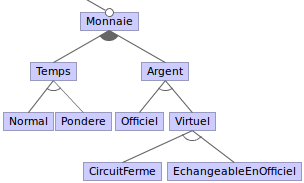
\includegraphics[scale=0.5]{Monnaie.png}}
\end{center}

\item [Monnaie]
\underline{Déf. :}  La monnaie utilisée dans une économie d'échange local est le moyen utilisé pour quantifier la valeur d'un bien ou un service.  Dans le dictionnaire des termes ( \ref{dicoMonnaie} ),  le principe de la monnaie a déjà été expliqué.   Ce feature englobe donc les différentes possibilités de monnaie.
\\ \underline{Justif. :}  Ce feature est optionnel car il se peut qu'une organisation n'utilise pas de monnaie.  Nous aurions alors un système d'échange gratuit.  Ceci existe déjà que ce soit pour des biens (les "donneries") ou services.  Si une monnaie est utilisée,  alors le système se limite à une seule.  Il est possible qu'une organisation aie plusieurs monnaies mais pour limiter la complexité de l'analyse et du framework,  nous nous limiterons au cas ou l'organisation utilise 0 ou 1 monnaie pour les échanges.
\newline

\item [Temps]
\underline{Déf. :}  Certaines organisations utilisent le temps comme monnaie d'échange.  La quantité est définie en unités temporelles habituelles (minutes,  heures,  jours, \dots ).  
\\ \underline{Justif. :}  Attention,  choisir cette monnaie comme moyen d'échange a un impact sur les possibilités futures d'échange.  En effet,  ce feature est à rejeter si l'on désire pouvoir échanger des biens/objets car utiliser cette monnaie représente du temps passé par une personne à réaliser une action.  Cela n'a donc pas de sens d'attribuer cette unité à un objet.
\newline

\item [Normal]
\underline{Déf. :}  Le temps peut être utilisé comme monnaie en représentant simplement le temps passé à réaliser le service échangé.
\\ \underline{Justif. :}  La plupart des organisations utilisant le temps comme monnaie d'échange pour des services se limitent à ce feature-ci.
\newline

\item [Pondéré]
\underline{Déf. :}  Ce feature laisse la possibilité à une organisation de personnaliser sa notion du temps.  Par exemple,  en considérant que certains services rapportent 2 fois le temps passé par la personne car celui-ci est plus rare.  
\\ \underline{Justif. :}  Ce feature n'est pas issu d'un constat de réalité mais plutôt d'une ouverture vers de nouvelles possibilités pour le futur.
\newline

\item [Argent]
\underline{Déf. :}  Ce feature désigne les monnaies plus classiques qui peuvent prendre une forme plus matérielle que le temps,  ou bien n'être que des monnaies virtuelles.
\\ \underline{Justif. :}  Ce feature est obligatoire si l'on désire pouvoir échanger des objets.  
\newline

\item [Officiel]
\underline{Déf. :}  Les monaies officielles regroupent,  tel que le nom l'indique,  les monnaies reconnues par des institutions publiques et englobent l'euro,  le dollar,  \dots.  
\\ \underline{Justif. :}  Pour des organisations désirant rester proches du système économique occidental "classique",  les monnaies officielles sont une évidence même.
\newline

\item [Virtuel]
\underline{Déf. :}  Les monnaies virtuelles englobent,  par opposition aux monnaies officielles,  les autres types d'argent qui peuvent exister mais ne seraient pas reconnues par des institutions publiques ou bien uniquement de façon très locale et dans un usage restreint.
\\ \underline{Justif. :}  Les systèmes d'échange local font partie des alternatives au système économique actuel qui a tendance à uniformiser et globaliser,  entre autres,  l'argent.  Il n'est donc pas rare de rencontrer des organisations qui ont créé leur propre monnaie complémentaire.  
\newline

% ================= 20 ===========
\item [CircuitFerme]
\underline{Déf. :}  Parmi les monnaies complémentaires,  certaines sont prévues pour ne pas être échangées afin,  par exemple,  de garder un aspect très local.  
\\ \underline{Justif. :}  
\newline

\item [EchangeableEnOfficiel]
\underline{Déf. :}  A l'inverse,  certaines monnaies peuvent être échangées contre de l'argent officiel.
\\ \underline{Justif. :}  Il est possible de déveloper un système de monnaie alternative (points ou autres) pour les échanges en interne et ceux-ci et de pouvoir les échanger auprès de l'organisation contre de l'argent réel.
\newline

\begin{center}
\fbox{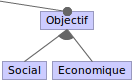
\includegraphics[scale=0.5]{Objectif.png}}
\end{center}

\item [Objectif]
\underline{Déf. :}  Ce feature doit être inclu afin de définir quel est l'objectif du modèle économique étudié.
\\ \underline{Justif. :}  Il est obligatoire de définir le ou les objectifs car cela peut avoir un impact sur l'outil final.  Plusieurs objectifs sont compatibles mais il en faut au moins 1.
\newline

\item [Social]
\underline{Déf. :}  Une organisation qui a pour but d'améliorer le bien-être des gens a un but social.
\\ \underline{Justif. :}  Beaucoup d'organisations actuelles ont princpalement un but social (ex. BuurtPensioen).
\newline

\item [Economique]
\underline{Déf. :}  Une organisation qui désire faire du profit grâce à l'orgnisation des échanges a un but économique.
\\ \underline{Justif. :}  Pour rendre ce genre de système rentable,  plusieurs exemples sont possibles : faire payer un abonnement aux utilisateurs,  faire payer chaque ou certains échanges, \dots
\newline

\item [Outil]
\underline{Déf. :}  Après avoir analysé le modèle économique du système d'échange local,  nous allons passer à l'outil.  On désigne ici les moyens matériels utilisés pour gérer l'économie locale.  Ce feature est optionnel car il est possible d'analyser un système sans que celui-ci ne possède d'outil.  
\\ \underline{Justif. :}  Le feature est à inclure si l'organisation possède un quelconque outil de gestion matérialisé,  c'est-à-dire au minimum sous forme papier.
\newline

\begin{center}
\fbox{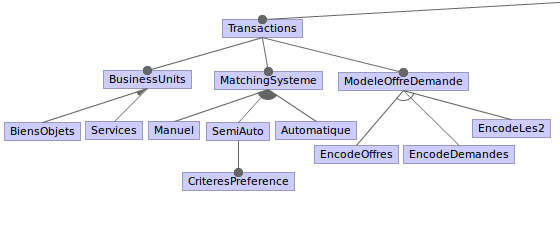
\includegraphics[scale=0.5]{Transactions.png}}
\end{center}

\item [Transactions]
\underline{Déf. :}  Les transactiosn sont les échanges possibles au sein de l'organisation.
\\ \underline{Justif. :}  Ce feature est obligatoire car si le système possède un outil de gestion,  le but premier de celui-ci sera de gérer les échanges entre acteurs.
\newline

\item [BusinessUnits]
\underline{Déf. :}  Les BusinessUnits représentent les unités échangées dans le système.
\\ \underline{Justif. :}  Ce feature est obligatoire car pour qu'il y ait échange,  il faut qu'il y ait quelque chose à échanger.
\newline

2 types d'unités sont échangeables : les \textbf{Biens ou Objet}s,  et les \textbf{Services}

%\item [BiensObjets]
%\underline{Déf. :}  Les biens ou objets sont des choses perceptibles par la vue et le toucher \footnote{\href{http://www.larousse.fr/dictionnaires/francais/objet/55366}{http://www.larousse.fr/dictionnaires/francais/objet/55366}}  et qui,  dans notre cas,  peuvent changer de propriétaire.
%\\ \underline{Justif. :}  Ce feature est à inclure si l'outil permet l'échange d'objets matérialisés. 
%\newline
%
%\item [Services]
%\underline{Déf. :}  Un service est un travail manuel ou intellectuel réalisé par une personne pour aider une ou plusieurs autres personnes.  Exemples de services : tâches ménagères,  jardinage,  baby-sitting,  \dots .
%\\ \underline{Justif. :} Ce feature est à inclure si 'lorganisation permet l'échange de services entre les acteurs. 
%\newline

% ================= 30 ===========
\item [MatchingSysteme]
\underline{Déf. :}  Le système de matching correspond aux fonctionnalités qui permettent de retrouver une offre lorsqu'on fait une demande ou vice-versa.  Les 3 possibilités de matching sont,  à chaque fois,  un choix à faire entre laisser plus de possibilités à l'utilisateur de choisir mais alors la recherche prend plus de temps,  ou à l'inverse,  accélérer la recherche pour l'utilisateur mais cela signifie lui laisser moins de choix.
\\ \underline{Justif. :}  Tous les systèmes d'échange local possèdent un système de matching qui sera,  pour le cas le moins automatisé,  totalement manuel.  Plusieurs systèmes peuvent cohabiter au sein du même système.
\newline

\item [Manuel]
\underline{Déf. :}  Un matching manuel signifie que les acteurs des échanges consultent et acccèdent à une liste des offres et/ou demandes manuellement,  sans qu'un tri préalable ait été effectué par l'outil.
\\ \underline{Justif. :} Ce feature est le fonctionnement le plus simple et celui laissant le plus de possibilités de choix aux acteurs. 
\newline

\item [Semi-auto]
\underline{Déf. :}  Un matching semi-automatique signifie que l'acteur qui désire effectuer une recherche dans les transactions encodées dans le système,  recevra une liste épurée de concordancees.  Cette liste est générée par le système sur base d'un ou plusieurs critères de préférence.
\\ \underline{Justif. :}  Ce feature offre moins de choix à l'utilisateur mais accélère la recherche d'une correspondance.
\newline

\item [Critère]
\underline{Déf. :}  Un critère de préférence correspond à un argument qui sera utilisé par le système pour effectuer un tri parmi toutes les possibilités de correspondance.
\\ \underline{Justif. :}  Un matching semi-automatique doit avoir au moins 1 critère sur lequel effectuer le tri de base.  Ce critère est lié à ce qui est recherché,  c'est-à-dire un bien ou un service,  ou à la transaction plus généralement.  Par exemple,  la date à laquelle un service doit avoir lieu peut être un critère de préférence ou bien,  pour toute transaction,  la distance à parcourir pour obtenir l'objet / réaliser la tâche,  peut également être un critère de préférence.   
\newline

\item [Automatique]
\underline{Déf. :}  Un matching automatique correspond à la fonctionnalité où le système recherche lui-même une correspondance dans les offres ou demandes enregistrées dans le système.  L'acteur n'a alors qu'une seule possibilité de correspondance.  Les critères utilisés pour faire correspondre les transactions sont internes au système.
\\ \underline{Justif. :}  Ce feature amène un système très efficace mais très peu tolérant des exigences des utilisateurs.  
\newline

\item [ModeleOffreDemande]
\phantomsection
\label{featOD}
\underline{Déf. :}  Le modèle d'offre et demande correspond aux fonctionnalités présentes dans l'outil pour faire savoir au système que l'on recherche ou que l'on propose un bien ou un service.  Par exemple,  les sites de type eBay,  2ememain et autres,  ne permettent l'encodage que des offres.  Si un utilisateur désire acquérir un objet,  il n'a pas la possibilité d'encoder sa recherche dans le site,  il doit chercher et essayer de trouver ce qui correspond le mieux à ses besoins.  Ce feature représente les actions possibles pour un acteur du système (enregistré ou non,  administrateur ou non,  à voir selon les autres features décrits ci-après).  
\\ \underline{Justif. :}  Ce feature est important à définir car l'outil peut être tout à fait différent selon les possibilités offertes aux acteurs.  Par facilité pour l'élaboration des contraintes décrites plus loin,  3 features sont disponibles mais 1 seul peut être choisi.  Soit on encode les offres,  soit les demandes,  soit les 2.  Cette notation remplace une cardinalité de 1 ou + avec 2 éléments possibles mais ne change pas sa signification.
\newline

\item [EncodeOffres]
\underline{Déf. :}  Encoder les offres implique que l'acteur d'une transaction puisse insérer dans le système une description du bien ou service qu'il est prêt à échanger avec un autre acteur.  Conformément à la définition donnée,  l'acteur se trouve alors dans la position du fournisseur (\ref{dicoTermes}).
\\ \underline{Justif. :}  Beaucoup de sites de commerce en ligne fonctionnent de la sorte ( \href{http://www.befr.ebay.be/}{eBay\copyright} et autres )
\newline

\item [EncodeDemandes]
\underline{Déf. :}  Encoder les demandes implique que l'acteur d'une transaction puisse insérer dans le système une description du bien ou service qu'il aimerait pouvoir obtenir d'un autre acteur.   Celui-ci serait donc dans la position de bénéficiaire ( \ref{dicoTermes}).
\\ \underline{Justif. :}  
\newline

\item [EncodeLes2]
\underline{Déf. :}  Les 2 possibilités précitées peuvent coexister dans un même système.
\\ \underline{Justif. :}  Feature à inclure si le système offre les 2 possibilités expliquées ci-dessus.
\newline

\begin{center}
\fbox{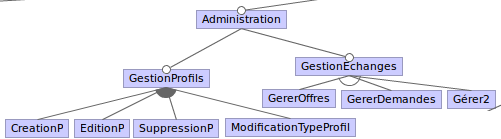
\includegraphics[scale=0.5]{Administration.png}}
\end{center}

\item [Administration]
\underline{Déf. :}  L'existence d'un système d'administration permet d'accéder à des fonctionnalités avancées de l'outil qui ne sont pas accessibles aux utilisateurs.
\\ \underline{Justif. :}  Beuacoup d'outils ont une possibilité d'administration mais ce n'est pas une obligation.  Le feature est donc optionnel.  De plus,  les 2 sous-arbres sont optionnels car ils représentent une modification des données du système mais des outils pourraient avoir des fonctionnalités d'administration plus orientées "technique" (modification du texte de description dans une page, \dots).
\newline

% ================= 40 ===========
\item [GestionProfils]
\underline{Déf. :}  Une des fonctionnalités administratives peut être la gestion des comptes d'utilisateurs.
\\ \underline{Justif. :}  Inclure ce feature signifie qu'il est possible de modifier les données qui présentent les acteurs dans le système.
\newline

\item [CreationP - EditionP - SuppressionP]
\underline{Déf. :}  La création/modificiation/suppression d'un profil permet à un administrateur d'enregistrer/supprimer lui-même une personne dans le système ou de modifier ses informations.
\\ \underline{Justif. :}  Certains outils restreignent l'inscription à une personne physique elle-même,  par exemple,  via l'utilisation d'un lecteur de carte d'identité électronqiue pour éviter les comptes anonymes.  La fonctionnalité de création ou modification via l'administration peut donc être disponible,  ou pas.  La suppression peut aussi ne pas être autorisée si on désire que les utilisateurs gardent un seul et même compte "pour toujours". 
\newline

\item [ModificationTypeProfil]
\phantomsection
\label{featTypes}
\underline{Déf. :}  Certains outils exigent que les membres fassent partie de différents types de profil.  Par exemple,  dans BuurtPensioen,  il existe un système de "membre vérifié".  Les acteurs qui s'inscrivent sont d'abord du type "non-vérifié" et suite à quelques démarches administratives et données particulières encodées,  ils peuvent accéder au statut de "vérifié".  
\\ \underline{Justif. :}  Ce feature n'a de sens que si le système de types de profils (voir features Utilisateurs \ref{featUtils}).
\newline

\item [GestionEchanges]
\underline{Déf. :}  Une fonctionnalité importante de l'administration peut concerner des modifications sur les offres ou demandes encodées dans le système.
\\ \underline{Justif. :}  Tout comme pour la gestion des profils,  il est possible que l'on offre pas la possibilité de les biens ou services que les utilisateurs ont encodés.  Ce feature est donc optionnel.  S'il est présent,  alors 1 seul des 3 sous-arbre est possible.  Il s'agit du même pattern que pour le modèle des offres et demandes ( \ref{featOD} ).
\newline

\item [GérerOffres - GérerDemandes - Gérer2]
\underline{Déf. :}  Cette gestion peut concerner l'ajout/suppression d'offres ou demandes ainsi que de la modification des données relatives.  
\\ \underline{Justif. :}  Un exemple d'utilité à cette fonction est simplement la surveillance des annonces faites dans l'outil afin d'éviter les dérives telles que les arnaques ou trafics d'objets volés,  \dots .   
\newline

Nous allons maintenant analyser les fonctionnalités qui peuvent êtres offertes par un système de gestion des utilisateurs enregistrés.

\begin{center}
\fbox{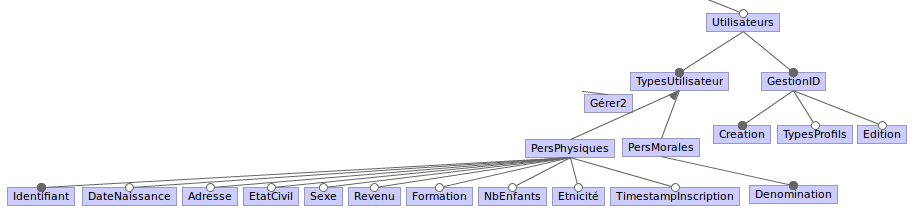
\includegraphics[scale=0.5]{Utilisateurs.png}}
\end{center}

\item [Utilisateurs]
\phantomsection
\label{featUtils} 
\underline{Déf. :}  Certains outils proposent aux acteurs des transactions de s'enregistrer dans l'outil,  par exemple,  via la création d'un compte ou profil unique.  
\\ \underline{Justif. :}  Même si beaucoup d'outils intègrent cette fonctionnalité,  ce feature est optionnel car un système d'échange peut tout à fait fonctionner sans que les acteurs n'aient la possibilité de s'enregistrer.  Par exemple,  le système de donnerie \footnote{\href{https://luna.agora.eu.org/listes/cgi-bin/mailman/listinfo/donnerie}{https://luna.agora.eu.org/listes/cgi-bin/mailman/listinfo/donnerie}} fonctionne par simple mailing liste classique.  Pour réaliser des transactions,  les acteurs communiquent entre eux via email.
\newline

% ================= 50 ===========
\item [TypesUtilisateurs]
\underline{Déf. :}  On fait ici référence aux publics cibles décrits dans le sous-arbre du modèle économique.  La différence est notée ici car les données retenues ne sont pas les mêmes selon les cas.
\\ \underline{Justif. :}  Ce feature est obligatoire car,  si l'outil intègre un système d'utilisateurs enregistrés (le feature supérieur),  il faut pouvoir s'enregistrer pour au moins 1 type d'utilisateur.   C'est pourquoi la cardinalité pour les fils est de 1 ou plus.
\newline

Le sous-arbre de ce feature est comparable au feature \textbf{PublicCible}.  On y retrouve les \textbf{PersonnesPhysiques} et \textbf{PersonnesMorales} ainsi que les informations que le système peut enregistrer à leur propos.

%\item [PersPhysiques]
%\underline{Déf. :}  Ce feature représente la possibilité pour des personnes physiques de s'enregistrer.  
%\\ \underline{Justif. :}  Inclure ce feature signifie qu'il faut pouvoir être identifié de façon unique dans le système.  Pour cela,  le feature "Identifiant" est obligatoire mais d'autres caractéristiques peuvent être encodées en plus.  
%\newline
%
%\item [Identifiant]
%\underline{Déf. :}  L'identifiant est la donnée de référence qui caractérise chaque acteur de façon unique dans le système.   Il peut s'agir d'un surnom unique,  du numéro de carte d'identité,  ou autre.
%\\ \underline{Justif. :}  L'identifiant est obligatoire si les personnes physiques sont incluses dans les profils.  
%\newline
%
%\item [DateNaissance - Adresse - EtatCivil - Sexe - Revenu - Formation - NbEnfants - Ethnicité - TimestampInscription]
%\underline{Déf. :}  Toutes ces informations sont liées à la demande faite par \href{http://www.vub.ac.be/EDWE/index.php?option=com_content&task=view&id=82}{Liesbeth De Donder} d'intégrer autant que possible des possibilités de statistiques relevantes dans le cadres des études menées à la VUB.  Notons que TimestampeInscription correspond à la date et à l'heure d'inscription de l'utilisateur afin de connaitre le moment où il s'est enregistré dans l'application.
%\\ \underline{Justif. :}  Il est intéressant de pouvoir inclure ces données dans le système si un système de statistiques peut être mis en place pour pouvoir récupérer et étudier ces données dans le cadre de recherches scientifiques.
%\newline
%
%\item [PersMorales]
%\underline{Déf. :}  Si le modèle économique vise,  entre autres,  des personnes morales et que l'outil intègre une gestion des utilisateurs,  alors un compte de type personne morale doit être possible.
%\\ \underline{Justif. :}  La distinction avec les personnes physiques est nécessaire car les données enregistrées ne sont pas les mêmes.
%\newline
%
%\item [Denomination]
%\underline{Déf. :}  La dénomination est une description texte courte qui représente la personne morale de façon unique.  
%\\ \underline{Justif. :}  Pour une personne morale,  on estime qu'un identifiant composé de la dénomination est la seule information de base nécessaire.  
%\newline

\item [GestionID]
\underline{Déf. :}  Ce feature représente les différentes possibilités existantes liées aux profils des acteurs enregistrés dans l'outil.  
\\ \underline{Justif. :}  Ce feature est obligatoire car si on intègre une gestion des utilisateurs,  il faut définir les actions possibles.  La seule action (donc feature) obligatoire est la création car sans elle,  il n'y aurait pas de gestion d'utilisateurs.  
\newline

\item [Creation]
\underline{Déf. :}  Ce feature représente la création d'un utilisateur dans le système.
\\ \underline{Justif. :}  Cette fonctionnalité est obligatoire car sans création initiale,   il n'y a pas de gestion. 
\newline

\item [TypesProfils]
\underline{Déf. :}   Ce feature représente la gestion des types de profils,  tel qu'expliqué dans les features d'administration ( \ref{featTypes} ).  Cette fois-ci,  il s'agit de la possibilité pour un membre de réaliser les démarches pour changer son type de profil.
\\ \underline{Justif. :}  Cette fonctionnalité peut être présente s'il n'y a pas de vérification faite par un administrateur.  De même,  elle peut être absente si seuls des gestionnaires sont aptes à changer le type de profil d'un membre (par exemple passer de "non-vérifié" à "vérifié").  
\newline

\item [Edition]
\underline{Déf. :}  L'édition d'un profil par un utilisateur correspond à la possibilité de modifier elle-même les informations liées à son profil.  
\\ \underline{Justif. :}  Ce feautre peut ne pas être inclus si,  par exemple,  l'outil a été créé pour ne fonctionner que sur base des informations d'une carte d'identité et qu'il n'est pas possible de les changer par la suite.
\newline

\begin{center}
\fbox{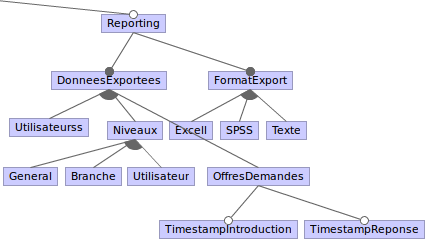
\includegraphics[scale=0.5]{Reporting.png}}
\end{center}

% ================= 60 ===========
\item [Reporting]
\underline{Déf. :}  Le reporting représente un sytème de statistiques offrant des informations sur les données encodées dans le système.  
\\ \underline{Justif. :}  Ce feature peut être présent et utile pour se rendre compte de l'utilisation du site mais n'est pas essentiel.
\newline

\item [DonneesExportees]
\underline{Déf. :}  On retrouve ici les différentes informations qui sont accessibles via le système de de reporting/statistiques
\\ \underline{Justif. :}  Ce feature est obligatoire car un système de reporting sans données exportées n'aurait pas de sens.  3 features sont possibles : l'export de données liées aux utilisateurs,  de celles des transactions ainsi que le niveau hierarchique que l'on désire couvrir.  Il est nécessaire d'en intégrer au moins 1 afin d'avoir des données à exporter.  

\item [Utilisateurs]
\underline{Déf. :}  Un des types de données qu'il peut être possible d'exporter concerne les utilisateurs.
\\ \underline{Justif. :}  Ce feature peut être utile afin de connaitre le public qui fréquente l'outil.
\newline

\item [Niveaux]
\underline{Déf. :}  On définit ici une portée des données qui seront exportées.  C'est à dire que l'on peut vouloir récolter des données issues de diffférentes parties de l'application.
\\ \underline{Justif. :}  Si ce feature est inclu et qu'au moins un des deux autres (utilisateurs ou offres/demandes),  alors le niveau définira l'origine des donées.  Si seuls les niveaux sont inclsu dans les données à exporter,  alors il s'agira d'inforamtions génériques sur ces niveaux.  
\newline

\item [General - Branche - Utilisateur]
\underline{Déf. :}  Ces trois niveaux signifient que l'on récolte des données qui concernent,  respectivement,  tout l'outil,  seulement une zone géographique limitée de l'outil ou uniquement les informations liées à un utilisateur précis.
\\ \underline{Justif. :}  Chaque niveau peut être utile pour analyser l'utilisation de l'outil.
\newline

\item [OffresDemandes]
\underline{Déf. :}  Les données concernant les offres et demandes concernent,  dans le cadre de cette analyse,  l'efficacité du système en terme de temps de réponse pour répondre aux besoins des utilisateurs.  
\\ \underline{Justif. :}  Pour analyser le temps de réponse par rapport aux transactions,  il est nécessaire de pouvoir retrouver le moment où la proposition de transaction a été introduite et où elle a été résolue si un système d'historique est mis en place.  
\newline

\item [TimestampIntroduction - TimestampReponse]
\underline{Déf. :}  Il s'agit,  ici,  du jour et de l'heure auxquels la transaction a d'abord été introduite puis résolue.
\\ \underline{Justif. :}  Ces 2 features sont fondamentalement optionnels mais si on désire pouvoir calculer le temps de réponse,  alors les deux dates et heures sont obligatoires.
\newline

% ================= 70 ===========
\item [FormatExport]
\underline{Déf. :}  Le format d'export correspond au type de support qui contient les données exportées.
\\ \underline{Justif. :}  Si des données peuvent être exportées,  alors il faut définir quel support sera utilisé.  Ce feature est donc obligatoire.
\newline

\item [Excell]
\underline{Déf. :}  Le support excell correspond à un fichier de type "classeur",  ou "tableur".  Typiquement,  un fichier dont l'extension peut être .xls,  .xlsx,  .csv,  ou encore .ods pour la version open-office.  Les fichiers respecteront bien sur les conventions liées à ces formats standardisés.
\\ \underline{Justif. :}  L'export au format excell peut être pratique pour une analyse de base via des graphiques se basant sur les données exportées.  Ce support est assez répandu mais reste limité pour un usage statistique avancé.   Plusieurs formats peuvent cohabiter dans le même outil.
\newline

\item [SPSS]
\underline{Déf. :}  SPSS\copyright est un logiciel de statistiques permettant une analyse plus avancée que les logiciels de bureautique de type "classeur".
\\ \underline{Justif. :}  Un export au format SPSS est intéressant pour alimenter les analyses réalisées dans le cadre d'études,  par exemple,  à la VUB.
\newline

\item [Texte]
\underline{Déf. :}  Le format texte est le plus simple.  Il correspond à un simple fichier sans structure standardisée.   Il est tout de même important de bien caractériser les données reprises.
\\ \underline{Justif. :}  Ce format est le plus simple et le plus facile à mettre en place mais offre moins de possibilités et facilités pour l'utilisation des données dans le futur.
\newline

\begin{center}
\fbox{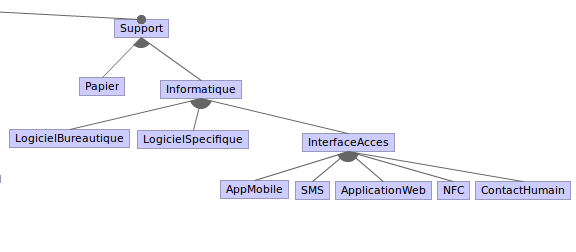
\includegraphics[scale=0.5]{Support.png}}
\end{center}

\item [Support]
\underline{Déf. :}  Ce feature désigne le support technique utilisé par l'outil.
\\ \underline{Justif. :}  Si un outil existe,  alors il doit avoir au moins 1 support pour exister.  Ce feature est donc obligatoire et au moins 1 des fils doit être inclus.
\newline

\item [Papier]
\underline{Déf. :}  Le support papier est le plus simple à mettre en place mais certainement le moins efficace.  Il implique qu'une personne centralise tous les documents.
\\ \underline{Justif. :}  Certaines organisations fonctionnent de la sorte,  souvent pour raison historiques.  Il peut s'agit,  par exemple,  d'un petit groupe de personnes et qui peut avoir grandi mais n'a pas changé d'outil.
\newline

\item [Informatique]
\underline{Déf. :}  Une manière plus efficace de s'organiser de nos jours passe par l'informatique,  au sens ethymologique du terme,  c'est-à-dire le traitement automatique des informations.  Plusieurs supports existent pour ce traitement automatisé.
\\ \underline{Justif. :}  Développer une solution informatique pour un outil de gestion est un investissement initial en temps (et souvent argent) assez conséquent mais rapidement rentabilisé si la solution est appropriée.  Remarquons que l'informatique fait gagner beaucoup de temps quand cela fonctionne comme prévu mais en fait perdre beaucoup dans le cas contraire.
\newline

\item [LogicielBureautique]
\underline{Déf. :}  Ce feature représente l'utilisation d'un logiciel tel que ceux des suites de bureautique (Microsoft Office \copyright ou OpenOffice).  On peut ainsi utiliser un tableur ou un système de gestion de base de données.
\\ \underline{Justif. :}  Ce type de logiciel est une bonne première approche d'un outil de gestion informatisée mais possède ses limites d'efficacité.
\newline

\item [LogicielSpecifique]
\underline{Déf. :}  Un logiciel spécifique est un logiciel développé dans le but de gérer une organisation telle que les économies d'échange local.  
\\ \underline{Justif. :}  Des exemples de ce type de logiciels ont été cités dans l'explication du problème (\ref{autresOrgas}).  
\newline

\item [InterfaceAcces]
\underline{Déf. :}  Ce feature regroupe les moyens techniques permettant d'accéder aux fonctionnalités de l'outil.
\\ \underline{Justif. :}  Plusieurs moyens peuvent coexister pour accéder à l'outil mais il en faut au minimum 1 sinon l'outil n'en est pas un.
\newline

% ================= 80 ===========
\item [AppMobile]
\underline{Déf. :}  Ce feature regroupe la possibilité d'accéder à l'outil via une application développée pour les smartphones ou tablettes ainsi que les sites web développés pour s'adapter aux smartphones et autres supports du même type.  
\\ \underline{Justif. :}   Ce type d'accès est utile pour augmenter l'interactivité avec les utilisateurs et peut,  par exemple,  permettre d'avoir des fonctionnalités de localisation par rapport au lieu encodé pour la transaction.
\newline

\item [SMS]
\underline{Déf. :}  Certaines fonctionnalités peuvent être accessibles via des SMS,  comme par exemple la validation d'une transaction dès que celle-ci est terminée.
\\ \underline{Justif. :}  Ce type d'interface peut aussi permettre plus d'interactivité avec les utilisateurs mais reste assez limitée en terme de fonctionnalités puisque les SMS se résument à des messages uniquement textuels. 
\newline

\item [ApplicationWeb]
\underline{Déf. :}  L'interface la plus répandue est l'interface web "classique".   On retrouve ici les applications web accessibles depuis un navigateur internet.  
\\ \underline{Justif. :}  Ce feature est certainement le plus commun à implémenter et utiliser et donc,  peut-être,  un choix de première interface de base.
\newline

\item [NFC]
\underline{Déf. :}  NFC signifie Near Field Communication.  Cette technologie consiste à une communication entre 2 appareils.  L'idée de base est similaire à la technologie bluetooth.
\\ \underline{Justif. :}  Cette technologie est en cours de développement pour l'application QOIN (\ref{QOIN}).  Cela peut être utile pour valider des transactions entre 2 acteurs lors de la rencontre physique de ceux-ci.
\newline

\item [ContactHumain]
\underline{Déf. :}  De nos jours,  on utilise beaucoup d'outils pour communiquer mais n'oublions pas les bases : un contact humain.  Ainsi on peut considérer que l'utilisateur peut utiliser l'outil via la rencontre avec une personne gérant l'outil.  
\\ \underline{Justif. :}  Cette possibilité est à prendre en compte car si le feature est inclus,  cela peut avoir un impact sur les méthodes d'administration possibles.  Le projet BuurtPensioen fait partie de ceux qui intègrent cette possibilité via des permanences par exemple.  
\newline

\begin{center}
\fbox{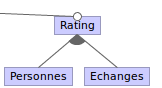
\includegraphics[scale=0.5]{Rating.png}}
\end{center}

\item [Rating]
\underline{Déf. :}  Le rating est un système qui permet de donner une note d'appréciation sur certains éléments de l'outil.
\\ \underline{Justif. :}  Ce feature peut être utile afin,  par exemple,  d'amener une certaine auto-régulation dans l'outil.
\newline

\item [Personnes]
\underline{Déf. :}  Un rating sur les personnes implique que l'on puisse commenter ou noter de façon quantitative un acteur de l'outil.  Ceci met alors en place un concept de "réputation" des acteurs.
\\ \underline{Justif. :}  Ce feature peut être une seconde façon d'amener de la sécurité en plus ou à coté du système de "type de profil" tel que cela existe pour le projet BuurtPensioen.
\newline

\item [Echanges]
\underline{Déf. :}  Un rating sur les échanges implique que l'on puisse commenter ou noter quantitativement une transaction.  De nouveau,  ceci peut permettre à d'autres utilisateurs de voir comment se passent les transactions avec les acteurs impliqués dans l'échange noté.
\\ \underline{Justif. :}  Ceci peut être utile d'un coté pour les utilisateurs mais également pour les gestionnaires afin d'évaluer la qualité des échagnes qui se déroulent via l'outil.
\newline

\end{description}

\subsubsection{Règles de composition}

Nous allons ici décrire les contraintes de composition du schéma.   Ces contraintes doivent être respectées pour obtenir un framework instancié fonctionnel.  Certaines sont plutôt d'ordre "philosophique",  c'est-à-dire qu'elles décrivent une contrainte pour qu'une instanciation soit cohérente.  D'autres sont d'ordre technique,  c'est-à-dire qu'il n'est pas possible d'instancier et programmer le modèle si on ne respecte la règle.

\underline{BusinessUnits > Biens/Objets REQUIRES Monnaie > Temps : }  Cette règle  signifie que cela n'a pas de sens d'échanger des objets matériels contre du temps.  Par contre,  une monnaie alternative peut être définie et utilisée.

\underline{GestionEchanges > chaque fils REQUIRES ModeleOffreDemande > le même fils présent : }  Cette règle est d'ordre technique.  Si,  par exemple,  si on désire qu'un administarteur puisse gérer la description d'une offre,  alors le système doit permettre d'encoder des descriptions d'offres.  Ceci s'applique pour chacun des fils. 

\underline{TypesUtilisateurs > chaque fils REQUIRES PublicCible > les mêmes fils présents : }  Cette contrainte est d'ordre philosophique et souligne que les utilisateurs qui s'enregistrent dans le système doivent faire partie du public cible de l'économique qui l'utilise.

\underline{Reporting > Niveaux > Utilisateurs REQUIRES Utilisateurs : }  Cette règle technique spécifie qu'il n'est pas possible d'avoir de statistiques par niveau si l'application ne possède pas cet élément de  hierarchie.

\underline{Rating > Personnes REQUIRES Utilisateurs : }  De même,  il n'est pas possible d'attribuer des appréciations aux comptes des utilisateurs si le système ne permet pas de créer des comptes.

\underline{Reporting REQUIRES Support > Informatique : } Pour que des statistiques puissent être faites,  il est nécessaire d'avoir un support informatique.  

\underline{Support > Informatique > Interface > Contact Humain REQUIRES Administration : }  Cette règle souligne que pour pouvoir intéragir avec le système au nom d'une tierce personne,  il faut pouvoir usurper son identité et donc utiliser un "mode administrateur".  

\underline{Administration > Gestion Profils REQUIRES Utilisateurs : } Cette contrainte souligne qu'il n'est pas possible de gérer des profils si le système n'offre pas de système de comptes d'utilisateur.

\subsubsection{Le feature model de Buurtpensioen}

Maintenant que le modèle des features est défini,  nous allons l'instancier au cas de Buurtpensioen,  et plus particulièrement à la solution proposée par le groupe d'étudiants,  afin de vérifier que le modèle est correct.

$\vcenter{\hbox{\fbox{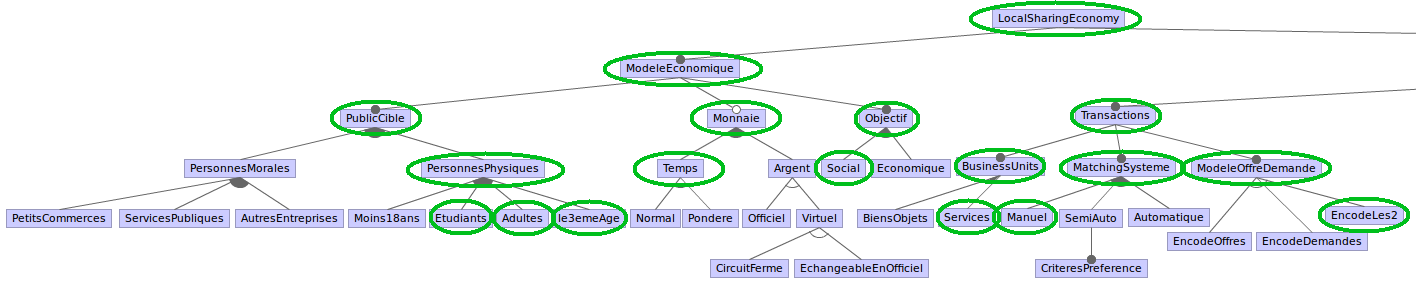
\includegraphics[scale=0.38,angle=90]{BP1.png} } }}$ \hspace{3 cm}
$\vcenter{\hbox{\fbox{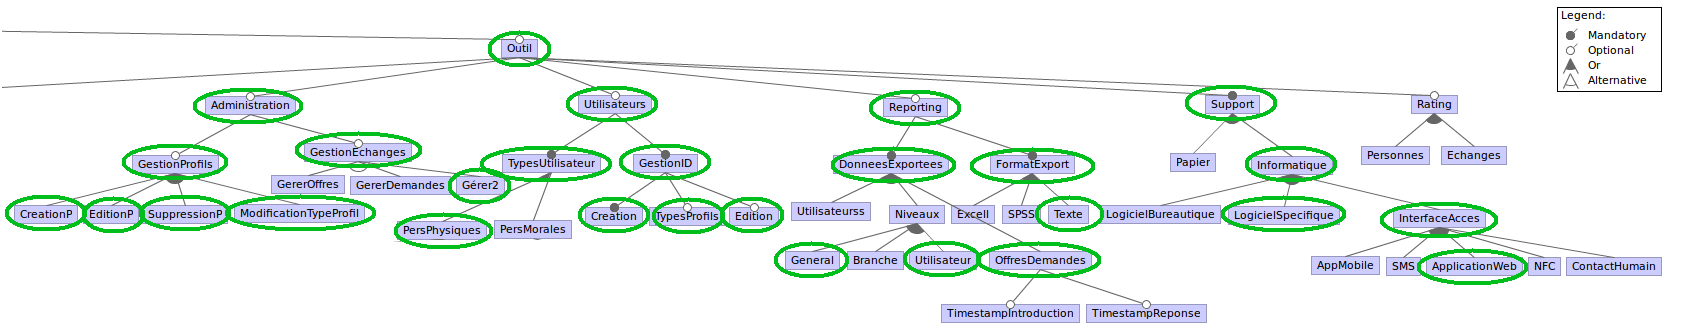
\includegraphics[scale=0.38,angle=90]{BP2.png} } }}$


\section{Developpement}

Maintenant que nous avons une analyse plus complète du domaine et plus particulièrement,  un arbre des features qui peuvent être intégrés dans le framework,  nous pouvons attaquer le développement.  Étant donné qu'il s'agit ici de programmation,  ce chapitre ne sera pas exhaustif du travail fourni mais permet de donner un aperçu de la façon de fonctionner.  Quelques exemples concrets et réels seront repris car nous éviterons de trainer sur des aspects trop techniques.  Nous allons commencer par décrire l'approche suivie pour la programmation du framework et ensuite,   nous passerons à la description du développement d'un feature choisi : la monnaie.  Celui-ci a été choisi car il permet de se rendre compte des différentes étapes pour l'implémentation d'un feature dans un projet Django.  Ce sera l'occasion de voir les techniques et patterns utilisés sans pour autant devoir expliquer trop de spécificités techniques liées à Django ou Python.  Notons que l'objectif ici est bien de modifier le code pour le rendre plus facile à appliquer par la suite.  Nous verrons dans le chapitre 7 (Validation) un exemple d'application concrète basée sur les features développés.   

\subsection{Approche}
Développer un framework est assez particulier et,  parce que nous partons d'un programme existant,  la méthode change quelques peu du cycle de développement habituel d'un logiciel.  Nous allons donc d'abord voir la façon dont nous allons fonctionner pour partir d'une solution existante spécifique et arriver à un framework plus générique,  dans le but de pouvoir ensuite dériver d'autres instances de ce framework.  Après avoir spécifié la méthode,  nous allons aborder rapidement un outil particulier qui a été utilisé pour le développement ainsi que les principales difficultés rencontrées pendant le processus.

\subsubsection{Développement d'un framework}

Le développement du framework va,  à l'instar de l'analyse,  se faire selon une démarche un peu particulière.  Pour illustrer celle-ci,  partons d'une comparaison.  Considérons qu'un logiciel est  comme un grand puzzle dont chaque pièce correspond à la partie du code liée à une fonctionnalité de l'application.  Dans le cas d'un framework,  par contre,  le puzzle possède des trous à l'endroit de certaines pièces et c'est en complétant ces trous que l'on obtient une application fonctionnelle.  Pour pouvoir développer les features un à un,  la démarche utilisée consiste donc à d'abord tenter de retrouver,  dans le projet,  toutes les parties du code qui concernent le feature dont il est question pour ensuite reprogrammer cette partie pour qu'il soit plus facile d'adapter cette fonctionnalité selon les cas prévus.

Le schéma suivant reprend les principales étapes du développement.  D'abord,  nous avons un logiciel foncionnel.  Ensuite,  on identifie les parties de code liées aux fonctionnalités (1 pièce = 1 fonctionnalité).  Après cela,  il faut transformer ce code pour qu'i soit facilement adaptable selon la situation.  On obtient ainsi les pièces en bleu.  Et enfin,  lorsqu'on désire instancier notre framework à un cas particulier,  on pourra programmer dans les parties nécessaires,  qui correspondent aux pièces en vert.

\begin{center}
\fbox{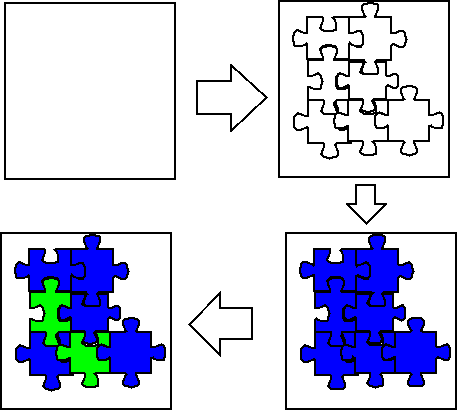
\includegraphics[scale=0.4]{puzzle.png}}
\end{center}

Enfin,  il est important de noter une difficulté particulière dans le cas du développement de notre framework.  En effet,  contrairement à une application orientée-objet classique,  notre framework est destiné au web.  Dès lors,  l'architecture est assez particulière et complique les choses pour toute la partie de retro-ingénierie du développement,  c'est-à-dire retrouver dans l'application,  les portions de code à traiter.  Cette complexité se rajoute aux diverses particularités de Django comme la description rigide du modèle de données ou les templates rédigés en HTML et quelques mots clés.

Pour faire face à cette complexité,  quelques outils peuvent aider lors du la rétro-ingénierie faite sur le logiciel de base (le travail du groupe 8) ainsi que pendant le développement.  Nous allons les décrire dans la prochaine section.

\subsubsection{Outils}

Pour nous aider dans le développement,  nous allons utiliser un simple script Python récupéré d'internet et légèrement adapté.  Son principe est assez simple,  il parcourt toute l'arborescence du projet et ouvre les fichiers un par un.  Pour chacun d'eux,  il recherche un mot clé passé en argument du script.  Après chaque fichier,  si le script a trouvé au moins 1 occurence,  le nom et le chemin du fichier sont affichés dans la console avec le nombre d'occurences dans le fichier.  Ceci permet de rapidement retrouver quelles parties de code utilisent une classe ou fonction que l'on recherche,  à partir du mot clé donné.  Par exemple,  si nous voulons retrouver tous les endroits où l'attribut first\_name (d'un utilisateur) est utilisé,  il suffit de se placer à la racine du projet et de lancer la commande : python3 search.py first\_name.  Dans ce cas-ci,  pour l'exemple,  nous avons précisé qu'il ne fallait lire que les fichiers python (nomDuFichier.endswith(".py") ) et le résultat est : 

\begin{lstlisting}
Found matches:
/media/maxime/Data/framework/newTest/branch/tests.py ['first_name', 'first_name', ......... , 'first_name', 'first_name']
/media/maxime/Data/framework/newTest/branch/views.py ['first_name', 'first_name', 'first_name', 'first_name']
/media/maxime/Data/framework/newTest/care4care/adapter.py ['first_name', 'first_name', 'first_name']
/media/maxime/Data/framework/newTest/care4care/lookups.py ['first_name']
/media/maxime/Data/framework/newTest/main/admin.py ['first_name', 'first_name', 'first_name', 'first_name']
/media/maxime/Data/framework/newTest/main/forms.py ['first_name', 'first_name']
/media/maxime/Data/framework/newTest/main/models.py ['first_name', 'first_name', 'first_name', 'first_name', 'first_name', 'first_name']
/media/maxime/Data/framework/newTest/main/tests.py ['first_name', 'first_name', ......... ,  'first_name']
/media/maxime/Data/framework/newTest/main/test_statistics.py ['first_name', 'first_name']
/media/maxime/Data/framework/newTest/main/views.py ['first_name', 'first_name', 'first_name', 'first_name', 'first_name']
\end{lstlisting}

Grâce à cela,  nous savons quels sont les fichiers qui utilisent cet attribut.  Et si nous le modifions,  nous devons vérifier/modifier à chaque endroit le code correspondand. 

Une autre astuce a été utilisée pour pouvoir débugger dans Django pendant le développement.  Il s'agit d'une simple instruction python permettant d'insérer l'équivalent d'un breakpoint. 
\begin{lstlisting}
import pdb; pdb.set_trace()
\end{lstlisting}
Lorsque le serveur arrive à ce point d'arrêt,  il se met en pause et une console s'ouvre.  
Dans la console,  on peut inspecter toutes les variables du programme en cours.  C'est très utile pour vérifier que les données sont bien correctes entre différents appels/pages/requêtes.

\subsection{Recherche et implémentation des features}

Pour le développement du framework,  nous allons donc démarrer de l'application du groupe 8 et tenter d'y retrouver les portions de code qui sont liées à des features précis.  L'objectif sera donc de partir du fait que,  dans notre arbre des features,  le groupe 8 a mis en place un feature feuille,  et l'objectif va être de transformer le programme pour correspond à un branchement supérieur.  Nous allons prendre un exemple avec le feature Temps pour arriver au feature Monnaie.  

\subsubsection{Feature Temps}

Le premier feature que nous allons analyser consiste en la monnaie utilisée.  Le travail du groupe 8 a appliqué le feature "Temps -> Normal",  c'est à dire que la monnaie utilisée dans l'outil est du temps.  L'objectif de cette partie consiste donc à retrouver les parties du code liées à la monnaie et de trouver une solution pour rendre ces parties plus génériques.

\paragraph{Etape 1 : localiser le feature}

\textbf{main/models.py}
\\%=================
La première chose à retrouver dans le code se trouve dans la description du modèle.  On y retrouve la classe User avec un attribut Credit ainsi qu'une méthode permettant de traduire en mots la valeur du crédit.
\\
\textbf{main/forms.py}
\\%================
Un autre endroit concerné par le feature de la monnaie est le fichier forms.py,  toujours dans l'application main.  On y retrouve la classe GIftForm qui permet d'afficher le formulaire de don de temps à un utilisateur.  La valeur de credit apparait dans la méthode clean\_amount de cettte classe et est liée à la variable amount,  définie comme un champ de formulaire au début de la classe.
\\
\textbf{main/views.py}
\\%================
Dans ce fichier,  on retrouve les crédits dans la méthode destinée à générer la vue pour consulter la page contenant ses informations liées au crédit.  Celle-ci est accessible depuis le menu de gauche,  lorsqu'un utilisateur est connecté.  Le template associé se situe dans /main/templates/credit/ .
\\
\textbf{main/urls.py et main/urls\_credits.py}
\\%==================================
On retrouve ici d'abord le fichier des urls de l'application main qui inclus les urls liées aux crédits via le fichier urls\_credits.py.  Ce dernier contient simplement une url qui redirige vers la page décrite au point précédent.
\\
\textbf{main/templates/credit/credit\_page.html}
\\%=====================================
Ce template html permet d'afficher toutes les informations générées via les fichiers précédents.
\\
\textbf{branch/views.py}
\\%=================
Au sein de ce fichier,   on retrouve les crédits dans une méthode manage\_success.  Celle-ci clôture un échange fructueux et les crédits interviennent pour réaliser l'échange de monnaie.  
\\
\textbf{templates/base.html}
\\%=====================
Dans ce fichier,  on retrouve le message qui apaprait lorsqu'on est connecté et qui affiche le crédit restant.  Attention : l'élément CSS utilisé par cet affichage est aussi utilisé pour le type de compte.   
\\
\textbf{Divers fichiers de rendu visuel}
\\%============================
On notera enfin que quelques pages plus statiques liées à la couche vue (rendu graphique et traduction).  Par exemple,  les traductions se retrouvent dans les fichiers locale/*langue*/LC\_MESSAGES/django.po avec *langue* pouvant prendre les valeurs "en" et "nl".  Ensuite,  on retrouve aussi quelques propriétés CSS dans static/css/style.css 
\newline
Ceci clôture le côté utilisateurs des crédits.  Il reste à repérer l'utilisation de ceux-ci dans les transactions.  
\\
\textbf{branch/models.py}
\\%=================
Pour cela,  nous allons à nouveau rechercher les propriétés dans les descriptifs des modèles. 
On y retrouve la classe Demand,  qui hérite de la classe Job.  Dans Demand,  2 éléments nous concernent : estimated\_time et real\_time.  
Dans la classe Offer,  il n'y a pas d'éléments liés à la monnaie.  Ceci est lié à un choix de design de l'outil.  En effet,   lorsqu'on désire encoder une offre dans le système,  on doit préciser une date et un type de service à rendre mais pas de crédit.  Il n'y a donc pas de crédit pour une offre telle quelle.
\\
\textbf{branch/views.py}
\\%=================
Ensuite,  dans le fichier views.py du même dossier,   nous retrouvons 2 occurences de real\_time.  
Une première fois lors de l'assignation de la valeur de success.time à demand.real\_time.  Cela signifie que,  avant que la demande puisse être enregistrée pour l'historique,  on enregistre la valeur du temps réellement pris pour le service qui est validé,  c'est à dire l'instance success.
La seconde fois concerne le formulaire de création de demande.  On retrouve donc l'élément dans la classe CreateDemandView où real\_time reçoit la valeur qui avait été estimée à la base.  
\\
\textbf{main/views.py}
\\%================
Enfin dans ce fichier,  on retrouve l'élément real\_time mais dans une méthode qui a déjà été signalée précédemment puisqu'il s'agit de l'affichage des crédits.
\\
\textbf{main/ajax/views.py}
\\%====================
L'élément real\_time est aussi utilisé pour créer des statistiques qui seront exportées au format JSON.
\\
\textbf{branch/forms.py}
\\%=================
Dans ce fichier,   l'élément estimated\_time apparait plusieurs fois dans 3 méthodes de création de formulaire : l'enregistrement et l'édition d'une demande d'aide ainsi que la réponse à une offre d'aide.
\\
\textbf{Fichiers de rendu visuel}
\\%=======================
3 fichiers de templates sont concernés par l'élément estimated\_time dans le dossier branch/templates/job/ : details\_demand.html,  need\_help.html et take\_offer.html.

\paragraph{Etape 2 : Refactoring vers un framework}

Maintenant que nous avons pu retrouver et comprendre les différentes portions de code qui sont impliquées dans le feature "Temps",  nous pouvons passer à l'action.  Pour ce faire,  allons suivre le cheminement général des appels dans l'application.  Mais juste avant,  précisons une dernière chose concernant la structure du logiciel dans lequel nous travaillons.  Il est important de rappeler que celle-ci est divisée en "sous-applications".  Chacune d'elle correspond à un sous-dossier du projet.  Les 2 sous-applications qui nous concernent sont Branch et Main.  Branch regroupe les fonctionnalités liées aux échanges et Main celles liées aux utilisateurs.  On remarque cette division en analysant le chemin des fichiers analysés ici avant (1 sous application = 1 sous-dossier).  

Les 2 types de points de départ que nous allons exploiter pour notre développement sont : les fichiers models.py qui définissent les modèles de données (1 par application),  et les templates,  qui contiennent des URL's qui représenteront les actions que les utilisateurs peuvent "activer".  

Pour le premier point qui concerne la description des modèles,  ce sont les fichiers models.py qui nous intéressent.  Dans l'analyse qui précède,  nous avions retrouvé 3 choses liées aux modèles : l'attribut Credit (et la fonction de type verbose qui va avec) dans la classe User,  définie dans l'application Main,  et les attributs estimated\_time et real\_time dans la classe Demand,  définie dans l'application Branch.  Le cas de la classe User est assez simple : nous allons simplement transformer la classe User ayant 1 attribut Crédit en 1 classe User qui peut hériter d'une autre classe,  qui elle-même possède l'attribut dont il est question.  Ceci permet de pouvoir hériter ou non de la classe (donc utilisation,  ou non,  d'une monnaie) ainsi que de définir dans une classe dédiée,  le comportement de la monnaie (dans le cas d'une monnaie alternative ou du temps ou autres).  

\begin{minipage}{.5\textwidth}
\begin{center} \textbf{Avant}\end{center}
\begin{lstlisting}
class User(AbstractBaseUser, PermissionsMixin, CommonInfo, VerifiedUser):
"""
Custom user class
"""
	email = models.EmailField(\_("Adresse email"), unique=False)
	...
	credit = models.IntegerField(default=0, verbose_name=\_("Credit restant")) # in minuts
	...
	def get_verbose_credit(self):
		credit = self.credit
		chunks = (...)
	...
	@models.permalink
	def get_absolute_url(self):
		return ('user_profile', (), {'user_id' : self.id})
\end{lstlisting} 
\end{minipage}
\hspace{0.3cm}
\begin{minipage}{.5\textwidth}
\begin{center} \textbf{Après}\end{center}
\begin{lstlisting}

class FWUser(models.Model):
    credit = models.IntegerField(default=0, verbose_name=_("Credit restant")) # in minuts   
    def get_verbose_credit(self):
        credit = self.credit
        chunks = (...)
        ...
    class Meta:
        abstract = True

class User(AbstractBaseUser, FWUser, PermissionsMixin, CommonInfo, VerifiedUser):
"""
Custom user class
"""
	...
\end{lstlisting} 
\end{minipage}


Le code décrivant le modèle pour les crédits des utilisateurs a ainsi été modifié pour être facilement adaptable selon le cadre dans lequel le logiciel sera utilisé.  Continuons donc notre cheminement à travers les appels dans l'application Django.  Nous allons faire la même chose pour les attributs liés aux demandes,  c'est-à-dire estimated\_time et real\_time dans branch/models.py.  

\begin{minipage}{.5\textwidth}
\begin{center} \textbf{Avant}\end{center}
\begin{lstlisting}
class Demand(Job):
    """ Representation of a demand """
    title = models.CharField( ...)
    ...
    estimated_time = models.IntegerField(verbose_name=_("Temps estime (en minutes)"), blank=True, null=True)
    real_time = models.IntegerField(verbose_name=_("Temps reel (en minutes)"), blank=True, null=True)
    ...
\end{lstlisting} 
\end{minipage}
\hspace{0.3cm}
\begin{minipage}{.5\textwidth}
\begin{center} \textbf{Après}\end{center}
\begin{lstlisting}
class FWMoney(models.Model):
    estimated_time = models.IntegerField(verbose_name=_("Temps estime (en minutes)"), blank=True, null=True)
    real_time = models.IntegerField(verbose_name=_("Temps reel (en minutes)"), blank=True, null=True)
    class Meta:
        abstract = True

class Demand(Job, FWMoney):
    """ Representation of a demand """
    title = models.CharField( ...)
    ...
\end{lstlisting} 
\end{minipage}


La description des classes liées à la base de données étant modifiée,  nous allons passer aux fichiers views.py,  qui correspondent à la couche Contrôlleur de l'application.  Selon l'analyse faite,  nous avons retrovué des utilisations des crédits,  entre autres,  pour l'affichage de la page décrivant les crédits de l'utilisateur,  lorsqu'il est connecté.  Cette même page permet également de faire un don de crédit à un autre utilisateur.  Pour l'affichage de formulaires,  le fichier views.py faire référence au fichier forms.py.  Ce dernier décrit les éléments de chaque formulaire et dans views.py,  nous importons ces descriptions et décrivons la logique derrière le formulaire.  Dès lors,  dans la sous-application Branch,  nous avons des crédits qui entrent en jeu (via les variable real et estimated\_time) dans la classe CreateDemandView(CreateView),  plus précisément dans la définition de la méthode : def form\_valid(self, form) ainsi que def manage\_success(request, success\_demand\_id).  La première classe est utilisé pour l'affichage du formulaire de crétaion d'une demande tandis que la seconde méthode,  elle,  est utilisée pour finaliser une transaction qui s'est déroulée avec succès.  Dans les 2 cas,  d'un point de vue technique,  la situation est différente de la modification des fichiers models.py.  En effet,  nous avons ici affaire à des descriptions de méthodes et il n'y a que quelques lignes de codes concernées par les crédits.  Etant donné que ces lignes en question sont des assignations de variable,  nous pouvons simplement décrire à chaque fois une méthode qui pourra être customisée et qui permettra de définir le comportement pour cette partie de l'application.  En concret,  voici quelques fragments de code pour mieux comprendre l'idée : 

\begin{minipage}{.5\textwidth}
\begin{center} \textbf{Avant}\end{center}
\begin{lstlisting}
class CreateDemandView(CreateView):
    def form_valid(self, form):
        ....
        form.instance.receiver = User.objects.get(pk=self.kwargs['user_id'])
        form.instance.real_time = form.instance.estimated_time
        return super(CreateDemandView, self).form_valid(form)

def manage_success(request, success_demand_id):
	...
          demand.real_time =  success.time
          demand.success = True
          demand.donor.credit += success.time
          demand.donor.save()
          demand.receiver.credit -= success.time
          demand.receiver.save()
\end{lstlisting} 
\end{minipage}
\hspace{0.3cm}
\begin{minipage}{.5\textwidth}
\begin{center} \textbf{Après}\end{center}
\begin{lstlisting}

def fw_man_success(demand, successTime):
    if successTime > 100000:
        successTime = 100000
    if successTime < 0:
        successTime = 0
    demand.real_time =  successTime
    demand.donor.credit += successTime
    demand.receiver.credit -= successTime  
    return demand

def fw_form_valid(form):
    form.instance.real_time = form.instance.estimated_time
    return form
...
...
class CreateDemandView(CreateView):
    def form_valid(self, form):
        ....
        form = fw_form_valid(form)
...
def manage_success(request, success_demand_id):
	...
         demand = fw_man_success(demand,  success.time)
...
\end{lstlisting} 
\end{minipage}

Concernant le fichier views.py de la sous-application Main (qui gère donc les utilisateurs),  nous retrouvons une seule méthode permettant d'afficher la page des crédits.  Étant donné que l'entièreté de la méthode est dédiée au feature temps,  il suffit d'isoler celle-ci pour la rendre plus accessible en cas de modification.  Pour cela,  nous avons simplement créé un fichier reprenant le code lié au framework.  Chaque fichier "couche" (models.py,  views.py,  forms.py) a donc un homonyme fw\_models.py,  fw\_views.py ,  etc .  Chacun de ces fichiers reprend les classes et méthodes adaptées dans le cadre du framework.  Cest le cas de la méthode def credits\_view(request) qui se retrouve entièrement dans le fichier "annexe".  Notons qu'il n'est pas toujours possible d'isoler les éléments dans un fichier séparé.  Reprenons l'exemple de models.py.  Dans ce cas là,  models.py importe les méthodes de fw\_models.py.  Mais fw\_models.py peut avoir besoin de la description de certains éléments de models.py.  Nous avons donc une boucle d'inclusion.  Ce qui implique que tout le code n'est pas systématiquement isolé dans un fichier différent.  

Pour la suite du développement,  nous allons suivre le second point de départ qui est donc les URL's.  Pour cela,  nous pouvons modifier les fichiers urls.py.  Il s'agit simplement,  pour chaque application,  de la liste des URL's prises en charges ainsi que la méthode ou la classe qui y est liée.  Pour la sous-application Branch,  il n'y a pas de référence directe au feature temps car les adresses gèrent les transactions.  Par contre,  dans la sous-application Main,  nous avons un fichier urls\_credits.py qui est inclus dans le fichier principal urls.py.  Ce fichier décrit une URL permettant d'accéder à la page d'affichage de crédits,  et fait référence à la méthode credits\_view,  que nous avons isolé précédemment.  Ainsi,  si vous voulons supprimer l'utilisation d'une monnaie dans le système,  cette référenc e peut être supprimée.  

Les derniers éléments à modifier pour mettre en place notre feature concernent la couche de vue de l'application.  Pour cela,  nous devons modifier les templates utilisés. Le premier est base.html.  Celui-ci,  comme son nom l'indique,  est le cannevas de base de toutes les pages de l'application.  C'est ce template qui permet,  par exemple,  d'afficher le menu supérieur et latéral gauche.  On y retrouve d'ailleurs l'affichage des crédits accumulés par l'utilisateur.  Cette référence doit être supprimée si on ne ddésire pas utliser de monnaie,  par exemple.  Pour faciliter l'adaptation,  nous allons isoler le code lié à cet affichage dans un "sous-template" auquel nous ferons appel dans base.html.  La même technique est utilisée pour le lien "Mes crédits" dans le menu latéral gauche.  Ci-dessous,  l'exemple illustré.  Ces fragments de code montrent comment ne pas afficher de crédits,  dans le cas d'une absence du feature monnaie,  donc.  

\begin{minipage}{.5\textwidth}
\begin{center} \textbf{Avant}\end{center}
\begin{lstlisting}
...
<p class="centered credit-p"><span class="credit-text"></span> {{ request.user.get_verbose_credit | safe }}</p>
...

<ul class="sub">
<li><span><a href=""> </a></span></li>
</ul>

...
\end{lstlisting} 
\end{minipage}
\hspace{0.3cm}
\begin{minipage}{.5\textwidth}
\begin{center} \textbf{Après}\end{center}
\begin{lstlisting}
...

...

...

Dans fw_base.html : 
<!--

<p class="centered credit-p"><span class="credit-text"></span> {{ request.user.get_verbose_credit | safe }}</p>

-->

Dans fw_base2.html : 
<!--

<ul class="sub">
     <li><span><a href=""> </a></span></li>
                </ul>

-->
\end{lstlisting} 
\end{minipage}

\subsubsection{Autres features}

\subsection{Architecture du framework}

TO DO




\section{Validation}

Groupe 8 | BuurtPensioen + 1 au customisation 

In this chapter, describe the experiment, benchmarks, case study or
other means of validation, which you conducted to prove that your
solution attains the objectives put forward in the introduction.

\begin{description}

\item[Method] Describe the details and approach of how you conducted
  your validation experiment(s).

\item[Results] Present the brute results obtained after having
  conducted the experiment, but don’t draw any conclusions yet.

\item[Analysis/discussion] Analyse the obtained results and discuss
  what conclusions you can draw from these results. If possible
  include statistical tests, charts, graphs to support your analysis.

\item[Threats to validity] Discuss all factors that may have
  negatively or positively influenced your results or that may cause
  the experiment to be difficult to replicate by others.

\item[Conclusion] Summarize the main findings of your work: what did
  you do, what was not covered, advantages, shortcomings, possible
  future work. Did you attain the initial objectives of the thesis?

  Make sure to revisit the initial problem statement and to point out
  explicitly how your solution addresses it. Also repeat the achieved
  contributions.

\end{description}

\section{Future Work}

Suite aux constats faits lors de la fin du chapitre précédent,  une première suite qui peut être donnée à ce projet consiste à terminer de débugger le framework afin d'éradiquer totalement la présence de petits bugs.  Ceci devrait être réglé pour la présentation orale de ce travail.  

De ce framework ``épuré'',  quelques améliorations pourraient être apportées au design mis en place pour la gestion des objets/services et offres/demandes.  En effet,  nous avons souligné lors du développement que le design actuel du modèle de ces classes n'était pas optimal et pouvait être amélioré.  Pour rappel,  nous avons abstrait certaines parties de code de la façon suivante : 

\vspace{1cm}
\begin{center}
\fbox{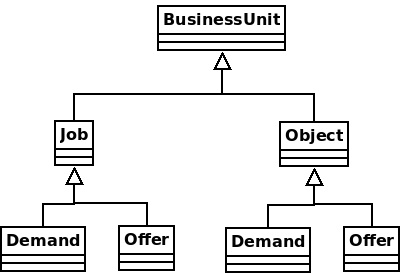
\includegraphics[scale=0.75]{modelsBU2.png}}
\end{center}
\vspace{1cm}

On remarque tout de suite que les classes Offre et Demande sont redondantes et nous avons ainsi une solution peu efficace.  Pour la suite du développement du framework,  il serait intéressant d'abstraire les offres et demandes dans une classe,  par exemple,  Transaction.  Ainsi,  le système réaliserait des échanges de Transactions de BusinessUnits.  Le schéma donnerait ce qui suit : 
\vspace{1cm}
\begin{center}
\fbox{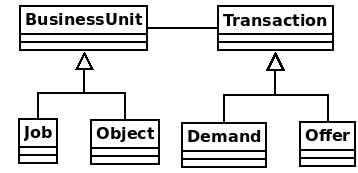
\includegraphics[scale=0.75]{newmodelsBU.png}}
\end{center}
\vspace{1cm}

Ce design permettrait de rendre le framework plus facilement adaptable pour prendre en compte l'existence,  ou non,  d'encoder des offres,  demandes,  concernant des objets ou transactions.  
\vspace{0.5cm}
Cependant,  la mise en place de ce design devrait,  selon moi,  amener un très important refactoring.  A peu près tout le code du fichier views.py (actuellement plus de 1200 lignes de code) devrait être refactoré mais pourrait amener à diminuer le nombre de classes/méthodes nécessaires à la coordination des actions.  Les templates sont également a réorganiser totalement pour pouvoir afficher correctement chaque type de transaction possible.   
\vspace{0.5cm}
 L'étape suivante peut consister en l'ajout de nouveaux features.  La méthode pour y parvenir devrait,  selon moi,  être un développement incrémental,  tel que commencé pour ce projet. En effet,  il est plus facile de suivre la démarche que nous avons décrite dans le chapitre sur le développement et ce,  pour chaque feature un par un.  Ceci semble nécessaire à la vue de la complexité du projet.  
\vspace{0.5cm}
D'une manière de plus globale,  il peut être intéressant d'envisager le concept de communauté de développeurs.  En effet,  ce framework est à destination d'organisations que l'on peut qualifier de ``transitionnaires'' et il a été développé sous licence open-source.  Ainsi,  ce serait une belle opportunité qu'un groupement se crée autour du framework afin d'une part pouvoir soutenir les organisations locales qui désirent instancier le framework,  et d'autre part,  développer de nouveaux features.  Il s'agit là,  selon moi,  d'une piste intéressante pour que ce projet soit utile à la société et utilisé par un maximum de projets locaux.  



\newpage
\section{Conclusion}

Arrivé à la fin de ce projet,  il est temps de faire le bilan des contributions de ce mémoire.  Tout d'abord,  la première partie de ce travail a consisté en une bonne dose d'analyse.  En effet,  le domaine des économiqes locales de partage est assez varié et quelques exemples de projets existants ont été repris dans le chapitre dédié à l'explication du problème.  Cette diversité a permis de donner du sens à la réalisation d'un framework plutôt qu'un projet plus classique.  En effet,  le framework offre plus de possibilités de personnalisation qu'un logiciel paramétrable,  tel que Cyclos.  Cette première étape d'analyse apporte un résultat intéressant pour le futur : un modèle des features réutilisable pour tout projet lié à ce domaine.  En effet,  cette analyse peut tout à fait être réutilisée et adaptée en vue de servir à la rédaction d'un cahier des charges d'un projet informatique.  Les définitions des features peuvent amener une première description des fonctionnalités nécessaires et le dictionnaire des termes est également une bonne source d'introduction au domaine.   
Lors du développement proprement dit,  les deux outils utilisés peuvent être considérés comme indispensables pour mettre en place un projet de cette ampleur.  En effet,  pour développer un framework,  une première étape de rétro-ingénierie est nécessaire.  D'autant plus dans notre cas puisque nous avons développé un framework destiné au web,  et donc organisé en couches composées de classes et méthodes qui s'entre-mêlent.  Ainsi,  pouvoir utiliser le debugger à des endroits clés ainsi que le script de recherche de mots clés semble indispensable.  

D'un point de vue temporel du déroulement du projet,  on distingue clairement 2 étapes : la construction du feature model d'une part,  et le développement d'autre part.  Chacune d'elle fût divisée en étapes parfois communes.  En effet,  dans les 2 cas,  il a fallut commencer par intégrer des notions théoriques.  Pour l'analyse,  il s'agissait des modèles de features,  que je ne connaissais pas auparavant.  Pour le développement,  plusieurs éléments ont dû être assimilés.  D'abord,  après avoir choisit le projet issu du groupe d'étudiants,  il a fallu s'approprier le framework Django,  ainsi que Python,  langage déjà abordé dans le cadre de certains cours mais en guise d'outil et non comme objet d'étude.  Pour Django,  le tutoriel officiel fût bien utile mais s'est malheureusement avéré insuffisant.  En effet,  une fois que l'on plonge dans le code d'un projet tel que celui qui a servi de base,  on se rend compte de la richesse de cet outil et de la complexité que l'utilisation de cette dernière peut amener.  De plus,  certains éléments du projets ou de Django en général utilisent des notions avancées de Python.  Ces 2 éléments mis ensemble m'amènent à plusieurs conclusions.  D'abord,  le développement d'un framework est plus difficile que pour un logiciel plus classique.  Dès lors,  le choix du langage qui sera utilisé par les programmeurs doit être adapté à leurs compétences.  Dans le cadre de ce projet,  la question s'est posée au moment du choix entre Cyclos et la solution du groupe d'étudiants.  Je dois bien reconnaitre que je ne m'attendais pas à devoir faire face à ce niveau de maitrise du langage.  L'autre conclusion concerne le framework Django.   En effet,  en repensant aux problèmes rencontrés pendant le développement,  je me rends compte qu'une partie était liée au fonctionnement de Django.  Dès lors,  je fais le lien avec le choix pré-cité et je pense que c'est peut-être (il faudrait mener une étude comparative pour pouvoir l'affirmer) une mauvaise idée de se baser sur un logiciel utilisant lui-même un framework,  dans le but de créer un framework pour un domaine particulier.  Je pense cela car,  lors de ce projet,  j'ai souvent été confronté à me demander si une erreur était liée à une mauvaise utilisation du langage Python ou bien de Django.  Ceci complique beaucoup la programmation,  et le problème empire si,  comme c'est mon cas,  le programmeur n'est pas expert dans au moins une des deux technologies évoquées (dans mon cas,  j'avais quelques connaissances en Python et découvrais totalement Django).  La leçon à retenir se trouve donc dans les choix qui sont posés pour ce qui servira de base au développement du framework.  Si on désire réutiliser un projet existant basé lui-même sur un framework,  il vaut mieux s'entourrer d'une équipe de connaisseurs dans les technologies liées.  Notons aussi que j'ai souligné,  au début du travail,  que le développement d'un framework se fait généralement à partir d'une solution existante.  Peut-être que ce principe peut être remis en cause si on désire absolument travailler avec un framework applicatif (c'est-à-dire qui fourni un environnement technique) et dans ce cas,  démarer le framework ``from scratch'',  pour reprendre l'expression utilisée au début de ce mémoire.

Enfin,  d'un point de vue plus personnel,  même si la difficulté rencontrée pour la programmation a été assez importante,  l'ensemble du mémoire fût aussi une belle opportunité de mettre en application de nombreux concepts abordés dans le cadre des cours de mon master en ingénierie logicielle tels que : la documentation d'une analyse de domaine,  la gestion de projets de développement informatique,  les designs patterns,  la programmation orientée objets,  etc.

En définitive,  ce travail a aussi donné des résultats intéressants dans divers domaines : l'analyse du  domaine des économies locales d'échange,  les outils pratiques pour le développement d'un framework ainsi que les bonnes pratiques de refactoring et enfin,  la conclusion que nous venons d'évoquer sur les choix faits avant de commencer la programmation.  

\newpage
\bibliographystyle{plain}
\nocite{*}
\bibliography{main}

\appendix

\section{Liens vers les annexes}
Les annexes sont à retrouver sur un GitHub créé pour l'occasion.

\textbf{Buurtpensioen requirements analysis}\\
\label{bpse}
\url{https://github.com/MaximeBiset/memoire/blob/master/Annexes/SE_requirements_analysis_Care4Care.pdf}

\end{document}

\endinput

Emacs config
------------
Local Variables:
TeX-master: t
End:
